\providecommand{\toplevelprefix}{../..}  % necessary for subfile bibliography + figures compilation to work, do not move this after documentclass
\documentclass[\toplevelprefix/book-main.tex]{subfiles}

\begin{document}

\chapter{Learning Linear and Independent Structures}
\label{ch:classic}\label{ch:linear-independent}

\begin{quote}
\hfill  ``{\em The art of doing mathematics consists in finding that special case which contains all the germs of generality}.''


$~$\hfill -- David Hilbert
\end{quote}
\vspace{5mm}

% \DP{Section 1: PCA (deterministic), PPCA (statistical), Matrix completion/RPCA (both). Add Power Iteration etc.}

% \DP{Section 2: Orthogonal Dictionary Learning (deterministic), Bernoulli-Gaussian ODL (statistical), allow different types of errors \(\implies\) ICA (statistical). Add power iteration (from \href{https://openreview.net/pdf?id=SJeY-1BKDS}{Simon's paper}).}

% \DP{Section 3: Sparse Coding with Overcomplete Basis (deterministic). Fast sparse coding algorithms like ISTA. If you give me the basis it's sparse recovery, otherwise you have to learn the basis (e.g. KSVD)}
% \yima{Actually, John's group has a series of work on learning over-complete dictionary with strong correctness and  theoretical guarantees.}

% \DP{write a historical note about how these variants are related to central problems}

%\DP{in ch3, note that diffusion generalizes PCA (use Peng's paper) as learning a denoiser at all levels}


\textit{Real data has low-dimensional structure.} To see why this is true, let us consider the unassuming case of static on a TV when the satellite isn't working. At each frame (approximately every \(\frac{1}{30}\) seconds), the RGB static on a screen of size \(H \times W\) is, roughly, sampled independently from a uniform distribution on \([0, 1]^{3 \times H \times W}\). In theory, the static \textit{could} resolve to a natural image on any given frame, but even if you spend a thousand years looking at the TV screen, it will not. This discrepancy is explained by the fact that the set of \(H \times W\) natural images takes up a vanishingly small fraction of the hypercube \([0, 1]^{3 \times H \times W}\). In particular, it is extremely low-dimensional, compared to the ambient space dimension. Similar phenomena occur for all other types of natural data, such as text, audio, and video. Thus, when we design systems and methods to process natural data and learn its structure or distribution, this is a central property of natural data which we need to take into account. %\sdb{do we need this example? we already have \ref{sec:intro-low-dimensionality}} \DP{I feel it's good to re-emphasize, it will connect to readers who skipped introduction. Plus this example is more tuned towards e.g. images and videos that will motivate the latter part of the book.}

Therefore, our central task is to learn a distribution that has low intrinsic dimension in a high-dimensional space. In the remainder of this section, we discuss several \textit{classical} methods to perform this task for several somewhat {\em idealistic} models for the distribution, namely models that are geometrically linear or statistically independent. While these models and methods are important and useful in their own right, we discuss them here as they motivate, inspire, and serve as a predecessor or analogue to more modern methods for more general distributions that involve deep (representation) learning.

Our main approach (and general problem formulation) can be summarized as:
\begin{tcolorbox}\centering
    \textbf{Problem:} \textit{Given one or several (noisy or incomplete) observations of a ground truth sample from the data distribution, obtain an estimate of this sample.}
\end{tcolorbox}
This approach underpins several classical methods for data processing, which we discuss in this chapter.
\begin{itemize}
    \item Section \ref{sec:lowrank} --- Principal Components Analysis (PCA): Given noisy samples from a distribution supported on {\em one low-dimensional subspace}, obtain an estimate of the true sample that lies on this subspace.
    \item  Section \ref{sec:ica} --- Complete Dictionary Learning and Independent Components Analysis (ICA): Given noisy samples from a distribution supported on {\em a union (\textit{not} the span) of few low-dimensional subspaces}, obtain an estimate of the true samples.
    \item Section \ref{sec:dictionary_learning} --- Sparse Coding and Overcomplete Dictionary Learning: Given noisy samples from {\em a distribution supported on combinations of a few incoherent vectors}, such as the coordinate axes, obtain an estimate of the true sample, which also has this property.
\end{itemize}
As we will soon reveal in later chapters, in the deep learning era, modern methods essentially adopt the same approach to learn.

In this chapter, as described above, we make simplifying modeling assumptions that essentially assume the data have geometrically (nearly, piece-wise) linear structures and statistically independent components. In Chapter \ref{ch:intro}, we have referred to such models of the data as ``analytical models''. These modeling assumptions allow us to derive efficient algorithms with provable efficiency guarantees\footnote{Both in terms of data and computational complexity.} for processing data at scale. However, they are imperfect models for often-complex real-world data distributions, and so their underlying assumptions only approximately hold. This means that the guarantees afforded by detailed analysis of these algorithms also only approximately hold in the case of real data. Nonetheless, the techniques discussed in this chapter are useful in their own right, and beyond that, serve as the ``special case with the germ of generality'', so to speak, in that they present a guiding motivation and intuition for the more general paradigms within (deep)  learning of more general distributions that we later address. %\sdb{feels it needs more adventurousness/authority (rely more on the really good opening quote for support)... also maybe be more clear about the structure of each section? (can also connect to the ``analytical models'' part of ch1)}\DP{took a stab}


% \yima{To be consistent with later chapters, we can cast all models and problems studied within the same compressive autoencoding framework:
% \begin{equation}
% \x \xrightarrow{\hspace{2mm} \mathcal{E} \hspace{2mm}}  \z \xrightarrow{\hspace{2mm} \mathcal{D} \hspace{2mm}}   \hat{\x}.    
% \end{equation}
% I would informally say that this chapter is for idealistic distributions which would allow either the encoder $\mathcal{E}$ or the decoder $\mathcal{D}$ to be {\em shallow and linear}. For the other opposite direction, it can be implemented via efficient (optimization) algorithms. I would even go further to specify for each of the model and problem, what exactly the associated encoding and decoding algorithm is. 
% }

% \yima{Guys, again, the purpose of this chapter is NOT to introduce these problems themselves. Our goal is to show how they all can be unified from the same perspective and within a common computational framework, that is also consistent with what is to come in the future chapters. }

% \sdb{We should take a cut at rewriting this introductory/motivation section along the lines of Yi's previous comment, to help focus the later presentations. Then rewrite and condense the PCA section accordingly. I am working on the section 2.2 rewrites for now.}

%wacwwwwwwwwwwwwwwwwwwwdadwThis chapter connects to the classic roots of data analysis with low-dimensional structures: geometrically linear, statistically independent.



%Extrinsic/intrinsic? Representation?

%The three (?) things that are echoed in the sequel:
%\begin{enumerate}
%    \item \textbf{What do we assume about reality?} Our model; mathematical
%        modeling.
%    \item \textbf{How do we compute with the model?} Simple models $\implies$
%        efficient computation.
%    \item \textbf{Does it work?} When the model assumption is met $\implies$ math proves
%        it works. (When it's ``okay'' $\implies$ bounded ``works'').
%\end{enumerate}
%Even if the model is too idealistic, its solution may convey the basic ideas that apply to the more general cases.

%\section{Modeling Low-dimensional Structures and Distributions}
%\pw{Some figures are missing on Page 56, Page 65}

\section{A Low-Dimensional Subspace} \label{sec:lowrank}

\subsection{Principal Components Analysis (PCA)}\label{sub:pca}

Perhaps the simplest modeling assumption possible for low-dimensional structure
is the so-called \textit{low-rank} assumption. Letting \(D\) be the dimension of
our data space, we assume that our data belong to a low-dimensional subspace of dimension \(d \ll D\), possibly plus some small disturbances. This ends up being a nearly valid assumption for some surprisingly complex data, such as images of handwritten digits and face data \cite{BasriR2003-PAMI} as shown in Figure \ref{fig:faces-digits}, yet as we will see, it will lend itself extremely well to comprehensive analysis. 

\begin{figure}
    \centering
    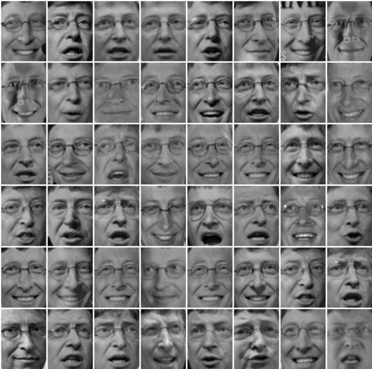
\includegraphics[width=0.4\linewidth]{\toplevelprefix/chapters/chapter2/figs/faces.png}
    \hspace{5mm} 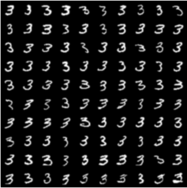
\includegraphics[width=0.395\linewidth]{\toplevelprefix/chapters/chapter2/figs/handwritten-digits.png}   
    \caption{Images of human faces and handwritten digits. Despite the seemingly large variety in their appearances, each set of those data spans (approximately) a very low-dimensional (nearly) linear subspace.}
    \label{fig:faces-digits}
\end{figure}

\paragraph{Problem formulation.}
To write this in mathematical notation, we represent a subspace \(\cS \subseteq \R^{D}\) of dimension \(d\)  by an orthonormal matrix \(\vU \in \O(D, d) \subseteq \R^{D \times d}\) such that the columns of \(\vU\) span \(\cS\). Then, we say that our data \(\{\vx_{i}\}_{i = 1}^{N} \subseteq \R^{D}\) have (approximate) low-rank structure if there exists an orthonormal matrix \(\vU \in \O(D, d)\), vectors \(\{\vz_{i}\}_{i = 1}^{N} \subseteq \R^{d}\), and \textit{small} vectors \(\{\veps_{i}\}_{i = 1}^{N} \subseteq \R^{D}\) such that 
\begin{equation}\label{eq:pca_dgp}
    \vx_{i} = \vU\vz_{i} + \veps_{i}, \quad \forall i \in [N].
\end{equation}
Here \(\veps_{i}\) are disturbances that prevent the data from being perfectly
low rank; their presence in our model allows us to quantify the degree to which
our analysis remains relevant in the presence of deviations from our model. The
true supporting subspace is \(\cS := \mathop{\mathrm{col}}(\vU)\), the span of
the columns of $\vU$. To process all we can from
this data, we need to recover \(\cS\); to do this it is sufficient to recover
\(\vU\), also called the \textit{principal components}. Fortunately, this is
a computationally tractable task named {\bf Principal Component Analysis}, and
we discuss now how to solve it.

Given data \(\{\vx_{i}\}_{i = 1}^{N}\) distributed as in \eqref{eq:pca_dgp}, we
aim to recover the model \(\vU\). A natural approach is to find the subspace
\(\vU^{\star}\) and latent vectors \(\{\vz_{i}^{\star}\}_{i = 1}^{N}\) which
yield the best approximation \(\vx_{i} \approx \vU^{\star}\vz_{i}^{\star}\). Namely, we aim to solve the problem 
\begin{equation}\label{eq:pca_sparse_recovery_problem}
    \min_{\tilde{\vU}, \{\tilde{\vz}_{i}\}_{i = 1}^{N}}\frac{1}{N}\sum_{i = 1}^{N}\norm{\vx_{i} - \tilde{\vU}\tilde{\vz}_{i}}_{2}^{2},
\end{equation}
where $\tilde{\vU}$ is constrained to be an orthonormal matrix, as above. We will omit
this constraint in similar statements below for the sake of concision.

\paragraph{Subspace encoding-decoding via denoising.}
To simplify this problem, for a fixed \(\tilde{\vU}\), we have (proof as exercise):
\begin{align}
    \min_{\{\tilde{\vz}_{i}\}_{i = 1}^{N}}\frac{1}{N}\sum_{i = 1}^{N}\norm{\vx_{i} - \tilde{\vU}\tilde{\vz}_{i}}_{2}^{2} 
    &= \frac{1}{N}\sum_{i = 1}^{N}\min_{\tilde{\vz}_{i}}\norm{\vx_{i} - \tilde{\vU}\tilde{\vz}_{i}}_{2}^{2} \\
    &= \frac{1}{N}\sum_{i = 1}^{N}\norm{\vx_{i} - \tilde{\vU}\tilde{\vU}^{\top}\vx_{i}}_{2}^{2}. 
\end{align}
That is, the optimal solution \((\vU^{\star}, \{\vz_{i}^{\star}\}_{i = 1}^{N})\)
to the above optimization problem has $\vz_i^{\star} = (\vU^{\star})^\top\vx_i$.

Now, we can write the original optimization problem in \(\tilde{\vU}^{\star}\)
and \(\{\tilde{\vz}_{i}\}_{i = 1}^{N}\) as an optimization problem just over
\(\tilde{\vU}\), i.e., to obtain the basis \(\vU^{\star}\) and compact codes
\(\{\vz_{i}^{\star}\}_{i = 1}^{N}\) it suffices to solve either of the two following equivalent problems:
\begin{equation}\label{eq:pca_equals_denoising}
    \min_{\tilde{\vU}, \{\tilde{\vz}_{i}\}_{i = 1}^{N}}\frac{1}{N}\sum_{i = 1}^{N}\norm{\vx_{i} - \tilde{\vU}\tilde{\vz}_{i}}_{2}^{2} = \min_{\tilde{\vU}}\frac{1}{N}\sum_{i = 1}^{N}\norm{\vx_{i} - \tilde{\vU}\tilde{\vU}^{\top}\vx_{i}}_{2}^{2}.
\end{equation}
Note that the problem on the right-hand side of \eqref{eq:pca_equals_denoising}
is a \textit{denoising} problem: given noisy observations \(\vx_{i}\) of
low-rank data, we aim to find the \textit{noise-free} copy of \(\vx_{i}\), which
under the model \eqref{eq:pca_dgp} is $\vz_{i}$. That is, the denoised input
$\hat{\vx}_i = \vU\vU^\top \vx_i$. Notice that this is the point on the subspace
that is closest to $\vx_i$, as visualized in \Cref{fig:pca-geometry}. Here by
solving the equivalent problem of finding the best subspace, parameterized by
the learned basis \(\vU^{\star}\), we learn an approximation to the
\textit{denoiser}, i.e., the projection matrix \(\vU^{\star}(\vU^{\star})^{\top} \approx \vU\vU^{\top}\) that projects the noisy data point $\x_i$ onto the subspace \(\cS\). %Denoising is one of the fundamental building blocks of high-dimensional data analysis, and we will discuss it often in this book, as many algorithms we will discuss are essentially denoising with respect to a particular data model (such as in \eqref{eq:pca_dgp}, but a bit more complicated). 

\begin{figure}
    \centering
    \begin{tikzpicture}
       \node (zero) at (0, 0) {};
       \node (u1) at (5, 1) {\(\vu_{1}\)};
       \draw[blue, ->, thick] (zero) -- (u1);
       \node[circle, inner sep=1.25pt, fill=red, draw=black] (x) at (3, 1.5) {};
       \node[circle, inner sep=1.25pt, fill=green, draw=black] (x_hat) at (3.2, 0.64)  {};
       \node at ($(x) + (0.5, 0.0)$) {\(\vx\)};
       \node at ($(x_hat) + (1, -0.2)$) {\(\hat{\vx} = \vu_{1}\vu_{1}^{\top}\vx\)};
       \draw[brown, ->, thick] (x_hat) -- (x);
       \node at (2.75, 1) {\color{brown}\(\varepsilon\)};
    \end{tikzpicture}
    \caption{\small \textbf{Geometry of PCA.} A data point $\vx$ (red) is projected onto the one-dimensional learned subspace spanned by the unit basis vector $\vu_1$ (blue arrow). The projection $\vU\vU^\top\vx = \vu_{1}\vu_{1}^{\top}\vx$ (green) is the denoised version of $\vx$ using the low-dimensional structure given by $\vu_{1}$, and $\boldsymbol{\varepsilon}$ (brown arrow) represents the projection residual or noise.}
    \label{fig:pca-geometry}
\end{figure}

Putting the above process together, we essentially obtain a simple encoding-decoding scheme that maps a data point $\vx$ in $\R^D$ to a lower-dimensional (latent) space $\R^d$ and then back to $\R^D$:
\begin{equation}
\x \xrightarrow{\hspace{2mm} \mathcal{E} = (\vU^\star)^\top \hspace{2mm}}  \z
    \xrightarrow{\hspace{2mm} \mathcal{D} = \vU^\star \hspace{2mm}}   \hat{\x}.  
\label{eqn:autoencoding-PCA}
\end{equation}
Here, $\vz \in \R^d$ can be viewed as the low-dimensional compact code (or
a latent representation) of a data point  $\x \in \R^D$ and the learned subspace
basis $\vU^\star$ as the associated codebook whose columns are the (learned)
optimal code words. The process achieves the function of denoising $\x$ by
projecting it onto the subspace spanned by $\vU^\star$.

\paragraph{Computing the subspace basis.}
For now, we continue our calculation. Let \(\vX = \mat{\vx_{1}, \dots, \vx_{N}} \in \R^{D \times N}\) be the matrix whose columns are the observations \(\vx_{i}\). We have (proof as exercise)
\begin{align}
    \argmin_{\tilde{\vU}}\frac{1}{N}\sum_{i = 1}^{N}\norm{\vx_{i} - \tilde{\vU}\tilde{\vU}^{\top}\vx_{i}}_{2}^{2}
    &= \argmax_{\tilde{\vU}}\frac{1}{N}\sum_{i = 1}^{N}\norm{\tilde{\vU}^{\top}\vx_{i}}_{F}^{2} \\ 
    &= \argmax_{\tilde{\vU}}\tr\rc{\tilde{\vU}^{\top}\bp{\frac{\vX\vX^{\top}}{N}}\tilde{\vU}}.
\end{align}
Thus, to compute the principal components, we find the orthogonal matrix
\(\tilde{\vU}\) which maximizes the term
\(\tr(\tilde{\vU}^{\top}(\vX\vX^{\top}/N)\tilde{\vU})\). We can prove via
induction that this matrix \(\vU^{\star}\) has columns which are the \textit{top \(d\) unit eigenvectors} of \(\vX\vX^{\top}/N\). We leave the whole proof to the reader in \Cref{exercise:principal-components-derivation}, but we handle the base case of the induction here. Suppose that \(d = 1\). Then we only have a single unit vector \(\vu\) to recover, so the above problem reduces to
\begin{equation}
    \max_{\tilde{\vu} \colon \norm{\tilde{\vu}}_{2} = 1} \tilde{\vu}^{\top}(\vX\vX^{\top}/N)\tilde{\vu}.
\end{equation}
This is the so-called \textit{Rayleigh quotient} of \(\vX\vX^{\top}/N\). By invoking the spectral theorem we diagonalize \(\vX\vX^{\top}/N = \vV\vLambda\vV^{\top}\), where \(\vV\) is orthogonal and \(\vLambda\) is diagonal with non-negative entries. Hence 
\begin{equation}
    \tilde{\vu}^{\top}(\vX\vX^{\top}/N)\tilde{\vu} = \tilde{\vu}^{\top}\vV\vLambda\vV^{\top}\vu = (\vV^{\top}\tilde{\vu})^{\top}\vLambda(\vV^{\top}\tilde{\vu}).
\end{equation}
Since \(\vV\) is an invertible orthogonal transformation, \(\vV^{\top}\tilde{\vu}\) is a unit vector, and optimizing over \(\tilde{\vu}\) is equivalent to optimizing over \(\tilde{\vw} := \vV^{\top}\tilde{\vu}\). Hence, we can write
\begin{equation}
    \tilde{\vu}^{\top}(\vX\vX^{\top}/N)\tilde{\vu} = \tilde{\vw}^{\top}\vLambda\tilde{\vw},
\end{equation}
whose optimal solutions \(\vw^{\star}\) among unit vectors are one-hot vectors whose only nonzero (hence unit) entry is in one of the indices corresponding to the largest eigenvalue of \(\vX\vX^{\top}/N\). This means that \(\tilde{\vu} = \vV\tilde{\vw}\), the optimal solution to the original problem, corresponds to a unit eigenvector of \(\vX\vX^{\top}/N\) (i.e., column of \(\vV\)) which corresponds to the largest eigenvalue.  Suitably generalizing this to the case \(d > 1\), and summarizing all the previous discussion, we have the following informal Theorem.
\begin{theorem}\label{thm:pca}
    Suppose that our dataset \(\{\vx_{i}\}_{i = 1}^{N} \subseteq \R^{D}\) can be written as 
    \begin{equation}
        \vx_{i} = \vU\vz_{i} + \veps_{i}, \qquad \forall i \in [N],
    \end{equation}
    where \(\vU \in \O(D, d)\) captures the \textit{low-rank structure},
    \(\{\vz_{i}\}_{i = 1}^{N} \subseteq \R^{d}\) are the \textit{compact codes}
    of the data, and \(\{\veps_{i}\}_{i = 1}^{N} \subseteq \R^{D}\) are small
    vectors indicating the deviation of our data from the low-rank model. Then
    the \textit{principal components} \(\vU^{\star} \in \O(D, d)\) of our
    dataset are given by the top \(d\) eigenvectors of \(\vX\vX^{\top}/N\),
    where \(\vX = [\vx_{1}, \dots, \vx_{N}] \in \R^{D \times N}\), and
    approximately correspond to the optimal linear denoiser:
    \(\vU^{\star}(\vU^{\star})^{\top} \approx \vU\vU^{\top}\).
\end{theorem}
We do not give explicit rates of approximation here as they can become rather
technical. In the special case that \(\veps_{i} = \vzero\) for all \(i\), the
learned \(\vU^{\star}\) spans the support of the samples \(\{\vx_{i}\}_{i
= 1}^{N}\). If in addition the \(\vz_{i}\) are sufficiently diverse (say,
spanning all of \(\R^{d}\)) then we would have perfect recovery:
\(\vU^{\star}(\vU^{\star}) = \vU\vU^{\top}\).
% \yima{The presentation of the above paragraph is somewhat awkward... Did we give the result for the $d=1$ case as an exercise or give the derivation somewhere? Or assume the student already knows that or at least give some reference? Also, maybe give a picture that illustrates the geometry?}


\begin{remark}
    In some data analysis tasks, the data matrix \(\vX\) is formatted such that each data point is a \textit{row} rather than a \textit{column} as is presented here. In this case the principal components are the top \(d\) eigenvectors of \(\vX^{\top}\vX/N\).
\end{remark}


\begin{remark}[Basis Selection via Denoising Eigenvalues]
    In many cases, either our data will not truly be distributed according to a subspace-plus-noise model, or we will not know the true underlying dimension \(d\) of the subspace. In this case, we have to choose \(d\); this problem is called \textit{model selection}. In the restricted case of PCA, one way to perform model selection is to compute \(\vX\vX^{\top}/N\) and look for instances where adjacent eigenvalues sharply decrease; this is one indicator that the index of the larger eigenvalue is the ``true dimension \(d\)'', and the rest of the eigenvalues of \(\vX\vX^{\top}/N\) are contributed by the noise or disturbances \(\veps_{i}\). Model selection is a difficult problem and, nowadays in the era of deep learning where it is called ``hyperparameter optimization'', is usually done via brute force or Bayesian optimization. %\sdb{``thresholding noise'' to learn $\vU$}
\end{remark}

\begin{remark}[Denoising Samples]
    The expression on the right-hand side of \eqref{eq:pca_equals_denoising}, that is,
    \begin{equation}\label{eq:orthogonal_denoising}
        \min_{\tilde{\vU}}\frac{1}{N}\sum_{i = 1}^{N}\norm{\vx_{i} - \tilde{\vU}\tilde{\vU}^{\top}\vx_{i}}_{2}^{2},
    \end{equation}
    is what's known as a \textit{denoising problem}, thusly named because it is an optimization problem whose solution \textit{removes the noise from the samples so it fits on the subspace}. Denoising --- learning a map which removes noise from noisy samples so that it fits on the data structure (such as in \eqref{eq:pca_dgp}, but maybe  more complicated) --- is a common method for learning distributions that will be discussed in the sequel and throughout the manuscript. Note that we have already discussed this notion, but it bears repeating due to its central importance in later Chapters.
\end{remark}

\begin{remark}[Neural Network Interpretation]
    If we do a PCA, we approximately recover the support of the distribution
    encoded by the parameter \(\vU^{\star}\). The learned denoising map then
    takes the form \(\vU^{\star}(\vU^{\star})^{\top}\). On top of being
    a denoiser, this can be viewed as a \textit{simple two-layer weight-tied
    linear neural network}: the first layer multiplies by
    \((\vU^{\star})^{\top}\), and the second layer multiplies by \(\vU^{\star}\), namely
    \begin{equation}
        \operatorname{denoise}(\vx) = \underbrace{\vU^{\star} \circ
        \underbrace{\id \circ \underbrace{(\vU^{\star})^{\top}\vx}_{\text{first ``layer''}}}_{\text{post-activation of first ``layer''}}}_{\text{output of ``NN''}}
    \end{equation}
    Contrasting this to a standard two-layer neural network, we see a structural similarity:
    \begin{equation}
        \operatorname{NN}(\vx) = \underbrace{\vW^{\star} \circ
        \underbrace{\mathrm{ReLU} \circ \underbrace{(\vU^{\star})^{\top}\vx}_{\text{first layer}}}_{\text{post-activation of first layer}}}_{\text{output of NN}}
    \end{equation}
    In particular, PCA can be interpreted as \textit{learning a simple two-layer
    denoising autoencoder},\footnote{In fact, as we have mentioned in the
    previous chapter, PCA was one of the first problems that neural networks
    were used to solve \cite{Oja1982SimplifiedNM,Baldi89}.} one of the simplest
    examples of a non-trivial neural network. In this framework, the
    \textit{learned representations} would just be \((\vU^{\star})^{\top}\vx \approx \vz\). In this way, PCA serves as a model problem for (deep) representation learning, which we will draw upon further in the monograph. Notice that in this analogy, the representations reflect, or are projections of, the input data towards a learned low-dimensional structure. This property will be particularly relevant in the future.
\end{remark}

\subsection{Pursuing Low-rank Structure via Power Iteration}\label{subsec:power iterations}

There is a computationally efficient way to estimate the top eigenvectors of \(\vX\vX^{\top}/N\) or any symmetric positive semidefinite matrix \(\vM\), called \textit{power iteration}. This method is the building block of several algorithmic approaches to high-dimensional data analysis that we discuss later in the Chapter, so we discuss it here. 

Let \(\vM\) be a symmetric positive semidefinite matrix. There exists an orthonormal basis for \(\R^{D}\) consisting of eigenvectors \((\vw_{i})_{i = 1}^{D}\) of \(\vM\), with corresponding eigenvalues \(\lambda_{1} \geq \cdots \geq \lambda_{D} \geq 0\). By definition, any eigenvector $\vw_i$ satisfies $\lambda_i \vw_i = \vM \vw_i$. Therefore, for any $\lambda_i > 0$, $\vw_i$ is a   ``fixed point'' to the following equation:
\begin{equation}
    \vw = \frac{\vM\vw}{\norm{\vM\vw}_{2}}.
    \label{eqn:PCA-fixed-point}
\end{equation}

\begin{theorem}[Power Iteration]
Assume that \(\lambda_{1} > \lambda_{i}\) for all \(i > 1\). If we compute the fixed point of  \eqref{eqn:PCA-fixed-point} using the following iteration:
\begin{equation}\label{eq:power_iteration}
    \vv_{0} \sim \dNorm(\vzero, \vone), \qquad \vv_{t + 1} \gets \frac{\vM\vv_{t}}{\norm{\vM\vv_{t}}_{2}},
\end{equation}
then, in the limit, \(\vv_{t}\) will converge to a top unit-norm eigenvector of \(\vM\).
\end{theorem}

\begin{proof} First, note that for all \(t\), we have 
\begin{equation}
    \vv_{t} = \frac{\vM\vv_{t - 1}}{\norm{\vM\vv_{t - 1}}_{2}} = \frac{\vM^{2}\vv_{t - 2}}{\norm{\vM\vv_{t - 1}}_{2}\norm{\vM\vv_{t - 2}}_{2}} = \cdots = \frac{\vM^{t}\vv_{0}}{\prod_{s = 1}^{t}\norm{\vM\vv_{s}}_{2}}.
\end{equation}
Thus, \(\vv_{t}\) has the same direction as \(\vM^{t}\vv_{0}\) and is unit norm, so we can write 
\begin{equation}
    \vv_{t} = \frac{\vM^{t}\vv_{0}}{\norm{\vM^{t}\vv_{0}}_{2}}.
\end{equation}
Because all the eigenvectors \(\vw_{i}\) of $\vM$ form an orthonormal basis for \(\R^{D}\), we can write 
\begin{equation}
    \vv_{0} = \sum_{i = 1}^{D}\alpha_{i}\vw_{i},
\end{equation}
where because \(\vv_{0}\) is Gaussian the \(\alpha_{i}\) are all nonzero with probability \(1\). Thus, we can use our earlier expression for \(\vv_{t}\) to write
\begin{equation}
    \vv_{t} = \frac{\vM^{t}\vv_{0}}{\norm{\vM^{t}\vv_{0}}_{2}} = \frac{\sum_{i = 1}^{D}\lambda_{i}^{t}\alpha_{i}\vw_{i}}{\norm{\sum_{i = 1}^{D}\lambda_{i}^{t}\alpha_{i}\vw_{i}}_{2}} = \frac{\sum_{i = 1}^{D}\lambda_{i}^{t}\alpha_{i}\vw_{i}}{\sum_{i = 1}^{D}\lambda_{i}^{t}\abs{\alpha_{i}}}. 
\end{equation}
Now, let us consider the case where \(\lambda_{1} > \lambda_{2} \geq \cdots \geq \lambda_{D} \geq 0\). (The case with repeated top eigenvalues goes similarly.) Then we can write
\begin{equation}
    \vv_{t} = \frac{\alpha_{1}\vw_{1} + \sum_{i = 2}^{D}(\lambda_{i}/\lambda_{1})^{t}\alpha_{i}\vw_{i}}{\abs{\alpha_{1}} + \sum_{i = 2}^{D}(\lambda_{i}/\lambda_{1})^{t}\abs{\alpha_{i}}}.
\end{equation}
Because \(\lambda_{1} > \lambda_{i}\) for all \(i > 1\), the terms inside the summation go to \(0\) exponentially fast, and the remainder is the limit 
\begin{equation}
    \lim_{t \to \infty}\vv_{t} = \frac{\alpha_{1}}{\abs{\alpha_{1}}}\vw_{1} = \sign(\alpha_{1})\vw_{1},
\end{equation}
which is a top unit eigenvector of \(\vM\). The top eigenvalue \(\lambda_{1}\) of \(\vM\) can be estimated by \(\vv_{t}^{\top}\vM\vv_{t}\), which converges similarly rapidly to \(\lambda_{1}\). 
\end{proof}

% \yima{How may the power iteration process be related to the denoising processing for the single Gaussian in Chapter 3?} \DP{there is not much of a connection, and we discuss this in Ch3}

To find the second top eigenvector, we apply the power iteration algorithm to \(\vM - \lambda_{1}\vv_{1}\vv_{1}^{\top}\), which has eigenvectors \((\vw_{i})_{i = 2}^{D}\) and corresponding eigenvalues \((\lambda_{i})_{i = 2}^{D}\). By repeating this procedure \(d\) times in sequence, we can very efficiently estimate the top \(d\) eigenvectors of \(\vM\) very quickly, for any symmetric positive semidefinite matrix \(\vM\). Thus we can also apply it to \(\vX\vX^{\top}/N\) to recover the top \(d\) principal components, which is what we were after in the first place. Notice that this approach recovers one principal component at a time; we will contrast this to other algorithmic approaches, such as gradient descent on global objective functions, in future sections.

% \DP{Remark: local iterative method to get components vs next section (and beyond) to optimize for global model: has historical roots and also algorithmic insights...}

% We discuss it in Section \ref{sec:power_iteration}. \sdb{do we really want to defer computation to the very end? (I agree that this is a good note to close on; I wonder if we could talk about computation for each example, then provide the unifying explanation/understanding at the very end? (which functions as a forward-looking conclusion to this chapter))}



\subsection{Probabilistic PCA}\label{subsec:probabilistic PCA}

Notice that the above formulation makes no statistical assumptions on the
data-generating process. However, it is common to include statistical elements
within a given data model, as it may add further enlightening interpretations
about the result of the analysis. As such, we ask the natural question:
\textit{what is the statistical analogue to low-dimensional structure?} Our answer is that a low-dimensional \textit{distribution} is one whose support is concentrated around a low-dimensional geometric structure. 

To illustrate this point, we discuss \textit{probabilistic principal component analysis (PPCA).} This formulation can be viewed as a statistical variant of regular PCA. Mathematically, we now consider our data as samples from a random variable \(\vx\) taking values in \(\R^{D}\) (also sometimes called a \textit{random vector}). We say that \(\vx\) has (approximate) low-rank statistical structure if and only if there exists an orthonormal matrix \(\vU \in \O(D, d)\), a random variable \(\vz\) taking values in \(\R^{d}\), and a \textit{small} random variable \(\veps\) taking values in \(\R^{D}\) such that \(\vz\) and \(\veps\) are independent, and
\begin{equation}
    \vx = \vU\vz + \veps.
\end{equation}
Our goal is again to recover \(\vU\). Towards this end, we set up the analogous problem as in Subsection \eqref{sub:pca}, i.e., optimizing over subspace supports \(\tilde{\vU}\) and random variables \(\vz\) to solve the following problem:
\begin{equation}
    \min_{\tilde{\vU}, \tilde{\vz}}\Ex\norm{\vx - \tilde{\vU}\tilde{\vz}}_{2}^{2}.
\end{equation}
Since we are finding the best such random variable \(\vz\) we can find its realization \(\vz(\vx)\) separately for each value of \(\vx\). Performing the same calculations as in Subsection \eqref{sub:pca}, we obtain %\sdb{weird notation here (it's a $\vz(\vx)$ inside the expectation? and $\vz$ reused?)}
\begin{equation}\label{eq:ppca_denoising}
    \min_{\tilde{\vU}, \tilde{\vz}}\Ex\norm{\vx - \tilde{\vU}\tilde{\vz}}_{2}^{2} = \min_{\tilde{\vU}}\Ex\min_{\tilde{\vz}(\vx)}\norm{\vx - \tilde{\vU}\tilde{\vz}(\vx)}_{2}^{2} = \min_{\tilde{\vU}}\Ex\norm{\vx - \tilde{\vU}\tilde{\vU}^{\top}\vx}_{2}^{2},
\end{equation}
again re-emphasizing the fact that the estimated subspace with principal components \(\vU^{\star}\) corresponds to a denoiser \(\vU^{\star}(\vU^{\star})^{\top}\) which projects onto that subspace. As before, we obtain 
\begin{align}\label{eq:PPCA}
    \argmin_{\tilde{\vU}}\Ex\norm{\vx - \tilde{\vU}\tilde{\vU}^{\top}\vx}_{2}^{2} 
    &= \argmax_{\tilde{\vU}}\Ex\norm{\tilde{\vU}^{\top}\vx}_{2}^{2} \\
    &= \argmax_{\tilde{\vU}}\tr(\tilde{\vU}^{\top}\Ex[\vx\vx^{\top}]\tilde{\vU}),
\end{align}
and the solution to the latter problem is just the top \(d\) principal components of the second moment matrix \(\Ex[\vx\vx^{\top}]\). Actually, the above problems are visually very similar to the equations for computing the principal components in the previous Subsection, except with \(\Ex[\vx\vx^{\top}]\) replacing \(\vX\vX^{\top}/N\). In fact, the latter quantity is an estimate for the former. Both formulations effectively do the same thing, and have the same practical solution --- compute the left singular vectors of the data matrix \(\vX\), or equivalently the top eigenvectors of the estimated covariance matrix \(\vX\vX^{\top}/N\). The statistical formulation, however, has an additional interpretation. Suppose that \(\Ex[\vz] = \vzero\) and \(\Ex[\veps] = \vzero\). We have
\begin{equation}
    \Ex[\vx] = \vU\Ex[\vz] + \Ex[\veps] = \vzero,
\end{equation}
so that \(\Cov[\vx] = \Ex[\vx\vx^{\top}]\). Now working out \(\Cov[\vx]\) we have 
\begin{equation}
    \Cov[\vx] = \vU\Cov[\vz]\vU^{\top} + \Cov[\veps] = \vU\Ex[\vz\vz^{\top}]\vU^{\top} + \Cov[\veps].
\end{equation}
In particular, if \(\Cov[\veps]\) is small, it holds that \(\Cov[\vx] = \Ex[\vx\vx^{\top}]\) is approximately a low-rank matrix, in particular rank \(d\). Thus the top \(d\) eigenvectors of \(\Ex[\vx\vx^{\top}]\) essentially summarize the whole covariance matrix. But they are also the principal components, so we can interpret principal component analysis as performing a low-rank decomposition of \(\Cov[\vx]\).

\begin{remark}
    By using the probabilistic viewpoint of PCA, we achieve a clearer and more quantitative understanding of how it relates to denoising. First, consider the denoising problem in \eqref{eq:ppca_denoising}, namely
    \begin{equation}
        \min_{\tilde{\vU}}\Ex\norm{\vx - \tilde{\vU}\tilde{\vU}^{\top}\vx}_{2}^{2}.
    \end{equation}
    It is not too hard to prove that if \(\veps\) is an isotropic Gaussian
    random variable, i.e., with distribution \(\veps \sim \dNorm(\vzero,
    \sigma^{2}\vI)\),\footnote{Other distributions work so long as they support
    all of \(\R^{D}\), but the Gaussian is the easiest to work with here.} then
    for \textit{any} solution \(\vU^{\star}\) to this problem, we have 
    \begin{equation}
        \vU^{\star}(\vU^{\star})^{\top} = \vU\vU^{\top}
    \end{equation}
    and so the true supporting subspace, say \(\cS \doteq \mathop{\mathrm{col}}(\vU)\), is
    recovered as the span of columns of \(\vU^{\star}\), since 
    \begin{equation}
        \cS = \mathop{\mathrm{col}}(\vU) = \mathop{\mathrm{col}}(\vU\vU^{\top})
        = \mathop{\mathrm{col}}(\vU^{\star}(\vU^{\star})^{\top})
        = \mathop{\mathrm{col}}(\vU^{\star}).
    \end{equation}
    In particular, the learned \textit{denoising map} \(\vU^{\star}(\vU^{\star})^{\top}\) is an orthogonal projection onto \(\cS\), pushing noisy points onto the ground truth supporting subspace. We can establish a similar technical result in the case where we only have finite samples, as in \Cref{thm:pca}, but this takes more effort and technicality. Summarizing this discussion, we have the following informal Theorem.
\end{remark}


\begin{theorem}\label{thm:ppca}
    Suppose that the random variable \(\vx\) can be written as
    \begin{equation}
        \vx = \vU\vz + \veps
    \end{equation}
    where \(\vU \in \O(D, d)\) captures the \textit{low-rank structure}, \(\vz\)
    is a random vector taking values in \(\R^{d}\), and \(\veps\) is a random
    vector taking values in \(\R^{D}\) such that \(\vz\) and \(\veps\) are
    independent, and \(\veps\) is small. Then the \textit{principal components}
    \(\vU^{\star} \in \O(D, d)\) of our dataset are given by the top \(d\)
    eigenvectors of \(\Ex[\vx\vx^{\top}]\), and approximately correspond to the
    optimal linear denoiser: \(\vU^{\star}(\vU^{\star})^{\top} \approx \vU\vU^{\top}\).
\end{theorem}

% \sdb{maybe more discussion on the conceptual significance of the denoising connection (correct errors... link to model selection and to score-based generative modeling... sample complexity and the conceptual insights). maybe do these for the case of $\vz$ Gaussian? (ICA chapter is ``non-Gaussian'')}

% The other examples in this Section will go similarly. We will introduce a motivating example, and geometric and statistical formulations of the problem.

\subsection{Matrix Completion}

%\DP{TODO: Insert a connection to deep learning; this transition isn't very good...}
%\yaodong{Why put the matrix completion here?}
In the previous Subsections, we discussed the problem of \textit{learning a low-rank geometric or statistical distribution}, where the data were sampled from a subspace with additive noise. But this is not the only type of disturbance from a low-dimensional distribution that is worthwhile to study. In this subsection, we introduce one more class of non-additive errors which become increasingly important in deep learning. Let us consider the case where we have some data \(\{\vx_{i}\}_{i = 1}^{n}\) generated according to \eqref{eq:pca_dgp}. Now we arrange them into a matrix \(\vX = \mat{\vx_{1}, \dots, \vx_{N}} \in \R^{D \times N}\). Unlike before, we do not observe \(\vX\) directly; we instead imagine that our observation was corrupted en route and we obtained 
\begin{equation}
    \vY = \vM \odot \vX,
\end{equation}
where \(\vM \in \{0, 1\}^{D \times N}\) is a \textit{mask} that is known by us, and \(\odot\) is element-wise multiplication. In this case, our goal is to recover \(\vX\) (from which point we can use PCA to recover \(\vU_{o}\), etc), given only the corrupted observation \(\vY\), the mask \(\vM\), and the knowledge that \(\vX\) is (approximately) low-rank. This is called \textit{low-rank matrix completion}.

There are many excellent resources discussing algorithms and approaches to solve this problem \cite{Wright-Ma-2022}. Indeed, this and similar generalizations of this low-rank structure recovery problem are resolved by ``robust PCA''. We will not go into the solution method here. Instead, we will discuss under what conditions this problem is \textit{plausible} to solve. On one hand, in the most absurd case, suppose that each entry of the matrix \(\vX\) were chosen independently from all the others. Then there would be no hope of recovering \(\vX\) exactly even if only one entry were missing and we had \(DN - 1\) entries. On the other hand, suppose that we knew that \(\vX\) has rank 1 exactly, which is an extremely strong condition on the low-dimensional structure of the data, and we were dealing with the mask
\begin{equation}
    \vM = \mat{\vone_{(D - 1) \times 1} & \vzero_{(D - 1) \times (N - 1)} \\ 1 & \vone_{1 \times (N - 1)} }.
\end{equation}
Then we know that the data were distributed on a line, and we know a vector on that line --- it is just the first column of the matrix \(\vY = \vM \odot \vX\). From the last coordinate of each column, also revealed to us by the mask, we can solve for each column since for each final coordinate there is only one vector on the line with this coordinate. Thus we can reconstruct \(\vX\) with perfect accuracy, and we only need a linear number of observations \(D + N - 1\). 

In the real world, actual problems are somewhere in between the two limiting cases discussed above. Yet the differences between these two extremes, as well as the earlier discussion of PCA, reveal a general kernel of truth:
\begin{quote}
    \centering
    \textit{The lower-dimensional and more structured the data distribution is, the easier it is to process, and the fewer observations are needed --- provided that the algorithm effectively utilizes this low-dimensional structure.}
\end{quote}
As is perhaps predictable, we will encounter this motif repeatedly in the remainder of the manuscript, starting in the very next section.

% An initial idea for solving this recovery problem is to set up an optimization problem, where the candidate solution matches the observation at all the unmasked indices and also has approximately low rank. This idea can be expressed by the following problem formulation:
% \begin{equation}
%     \min_{\substack{\vW \\ \vY = \vM \odot \vW}}\rank(\vW).
% \end{equation}
% However, this formulation runs into two issues:
% \begin{enumerate}
%     \item The \(\rank\) function is neither continuous nor convex, and thus it is computationally intractable to directly optimize.
%     \item The formulation may not properly account for approximately low-rank variables, which are ostensibly high rank but really just low rank plus noise.
% \end{enumerate}
% To address the first issue, we use the so-called \textit{convex relaxation} of the rank function, which is the nuclear norm \(\norm{\cdot}_{*}\), given by 
% \begin{equation}
%     \norm{\vA}_{*} = \tr([\vA^{\top}\vA]^{1/2})
% \end{equation}
% where \(\vB^{1/2}\) is the positive semidefinite square root. The three key properties of the nuclear norm are that (1) it is a convex function, (2) it forms an envelope for the rank function, i.e., \(\norm{\vA}_{*} \leq \rank(\vA)\) for all \(\vA\), providing an effective lower bound which can be optimized effectively, and (3) it is also efficient to compute. All three properties make it an attractive surrogate for the rank function in formulating the matrix completion problem. Thus, we use the following problem to recover \(\vX\):
% \begin{equation}
%     \min_{\substack{\vW \\ \vY = \vM \odot \vW}}\norm{\vW}_{*}.
% \end{equation}
% Finally, in order to address the second issue with the formulation, we use the Lagrangian form of this problem, obtaining 
% \begin{equation}
%     \min_{\vW}\bc{\frac{1}{2}\norm{\vY - \vM \odot \vW}_{F}^{2} + \lambda \norm{\vW}_{*}}.
% \end{equation}
% This formulation turns out to have attractive mathematical properties, as well as the conceptual grounding already discussed. 
% \sdb{this section does not really feel like it fits... maybe we could instead discuss the idea here of ``correcting gross errors (missing data) using low-dimensional structure'' via a basic conceptual discussion of how low-rank matrix completion isn't hopeless, then revisit it when talking about compressed sensing later?}

% \sdb{also note that the reason why general matrix completion is nontrivial is because model selection is much harder than in small-noise PCA/denoising... we don't talk about model selection in the current PCA part right now. if you take the model selection part out, the problem might become easy enough to write concretely about here}

% \DP{If we know the corruption, we can use PCA or matrix completion; if we don't, we can use Robust PCA. One paragraph.}


% \begin{itemize}
%     \item Classical examples: random noise \(\neq\) coherent images \(\implies\) coherent images have some serious structure
%     \item How to capture this structure?
%     \item Right data structures for images? sequences? (if we can motivate these to be subspaces, great, otherwise push to the end)
%     \item Naively: supported on the simplest low-dimensional objects we know how to think about (subspaces \(\implies\) PCA)
%     \item Less naively: generated by some easily describable process (sparse coding, dictionary learning, low-rank matrix completion)
%     \item Even less naively: belonging to a generic manifold
%     \item Data are sometimes drawn from a distribution
%     \item Simplest low-dimensional Gaussian distribution corresponds to subspace case
%     \item Less simple: Bernoulli-Gaussian corresponds naturally to dictionary learning, outer-product of Gaussian tall matrices corresponds to low-rank matrices
%     \item Generic low-dimensional probability distributions can be well-approximated by manifolds
%     \item Rest of the section: how to learn under these (simplest, less simple, general) assumptions --- classically
% \end{itemize}

% \DP{main goals for this subsection: connect geometric and statistical structures for data; talk about how data is structured at a high level (low-rank or low-dimensional manifold); gaussian/gaussian mixture assumption, approximation}

% \subsection{Learning a linear subspace via denoising} 
% Use the classic case of learning a single linear subspace to exemplify the general approaches to learn a low-dim model via compression (dimension reduction) from noising samples. Introduce the power-iteration algorithm... 

% Maybe also connect to the recent  diffusion perspective: When the diffusion-denoising process is specialized to the case of a low-rank Gaussian, it is equivalent to the classical PCA. Also the characteriztion of the number of samples needed.

% \subsection{Learning via completion and error correction}
% Might worth mentioning variatnts such as Matrix Completion, Robust PCA for learning low-dimensional linear models under more general notion of ``noise'' or ``perturbantion''. 

\section{A Mixture of Complete Low-Dimensional Subspaces}% and Complete Dictionary Learning } 
\label{sec:ica}
As we have seen, low-rank signal models are rich enough to provide a full picture of the interplay between low-dimensionality in data and efficient and scalable computational algorithms for representation and recovery under errors. 
These models imply a \textit{linear} and symmetric autoencoding pipeline \eqref{eqn:autoencoding-PCA}: 
\begin{equation*}
    \vz = \cE(\vx) = \vU^\top \vx, \quad \hat{\vx} = \cD(\vz) = \vU \vz,
\end{equation*}
which can be provably learned from finite samples of $\vx$ with principal component analysis (solved efficiently, say, with the power method) whenever the distribution of $\vx$ truly is linear.
This is a restrictive assumption---for as Harold Hotelling, the distinguished 20th century statistican,\footnote{By coincidence, also famous for his contributions to the development and naming of Principal Component Analysis \cite{Hotelling1933}.} objected following George Dantzig's presentation of his theory of linear programming for the first time \cite{Dantzig2002-eh},
\begin{quote}
\centering
    \textit{``...we all know the world is nonlinear.''}
\end{quote}


\begin{figure}
    \centering
    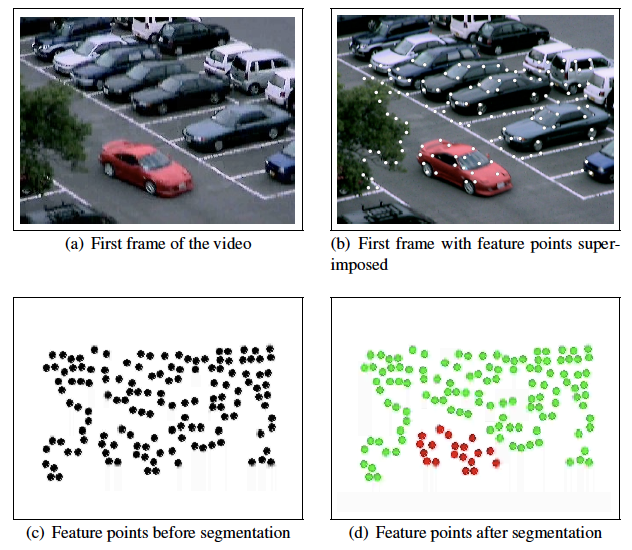
\includegraphics[height=0.35\linewidth]{\toplevelprefix/chapters/chapter2/figs/motion.png} \hspace{5mm}
    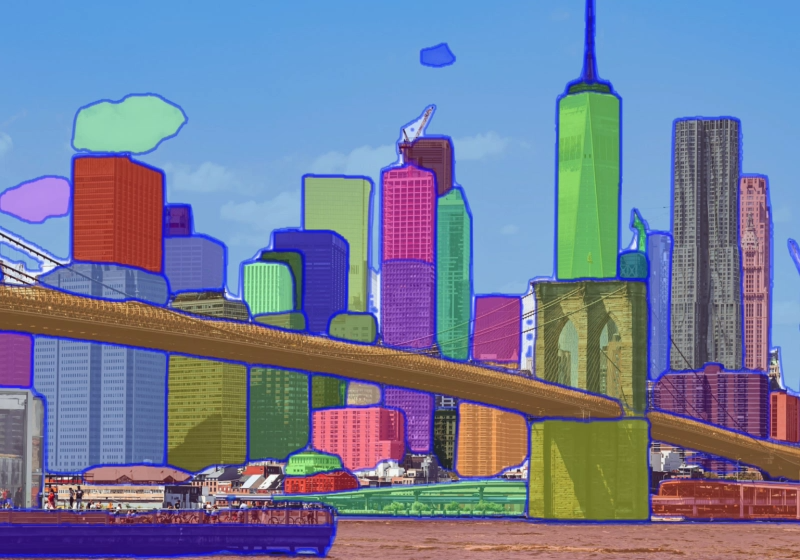
\includegraphics[height=0.349\linewidth]{\toplevelprefix/chapters/chapter2/figs/segment.png} 
    \caption{\textbf{Left:} features tracked on independently moving objects in a scene. \textbf{Right:} image patches associated with different regions of an image.}
    \label{fig:multiple-subspaces}
\end{figure}
Even accounting for its elegance and simplicity, the low-rank assumption is too restrictive to be broadly applicable to modeling real-world data. 
A key limitation is the assumption of a \textit{single} linear subspace that is responsible for generating the structured observations.
In many practical applications, structure generated by a \textit{mixture} of distinct low-dimensional subspaces provides a more
powerful and realistic model.
For example, consider a video sequence that captures the motion of several distinct objects, each subject to its own independent displacement (Fig.\ \ref{fig:multiple-subspaces} left). 
Under suitable assumptions on the individual motions, each object becomes responsible for an independent low-dimensional subspace in the concatenated sequence of video frames \cite{VidalR2004-ECCV}.
As another example, consider modeling natural images via learning a model for the distribution of \textit{patches}, spatially-contiguous collections of pixels, within an image (Fig.\ \ref{fig:multiple-subspaces} right). Unlike in the Eigenface example we saw previously, where images of faces with matched poses can be well-approximated by a single low-dimensional subspace, the patch at a specific location in a natural image can correspond to objects with very different properties---for example, distinct color or shape due to occlusion boundaries. Therefore, modeling the distribution of patches with a single subspace is futile, but a \textit{mixture} of subspaces, one for each region, performs surprisingly well in practice, say for segmenting or compressing purposes \cite{Mobahi-IJCV2011}.\footnote{We will return to this observation in Chapter \ref{ch:representation}, where we will show it can be significantly generalized to yield powerful representations for large-scale modern datasets.} We will see a concrete example in the next chapter (Example \ref{eg:image-segmentation}).



\begin{figure}
    \centering
    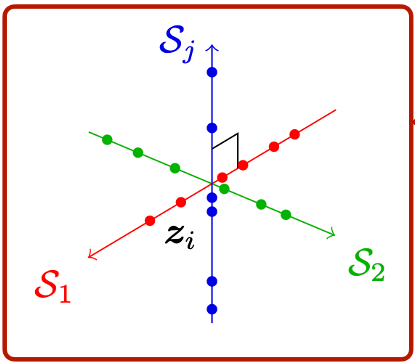
\includegraphics[height=0.35\linewidth]{\toplevelprefix/chapters/chapter2/figs/subspaces.png}
    \caption{Data on a mixture of low-dimensional subspaces, say $\mathcal{S}_j = \mbox{span}(\vU_j)$.}
    \label{fig:subspaces}
\end{figure}

In this section, we will begin by discussing the conceptual and algorithmic foundations for compressive autoencoding when the data distribution has a structure modeled by {\em a mixture of low-dimensional subspaces}, as illustrated in Figure \ref{fig:subspaces}. In this setting, the decoder mapping will be almost as simple as the case of a single subspace: we simply represent via
\begin{equation}\label{eq:mixture-subspaces-decoder-first-cut}
    \hat{\x} = \cD(\vz) = \left( \sum_{k=1}^K \pi_k(\vz)\vU_k \right) \vz,
\end{equation}
where $\pi_k : \R^d \to \set{0,1}$ are a set of \textit{sparse} weighting random variables, such that only a single subspace $\mathcal{S}_k = \mbox{span}(\vU_k) $ is selected in the sum.
However, the task of encoding such data $\vx$ to suitable representations $\vz$, and learning such an encoder-decoder pair from data, will prove to be more involved.

We will see how ideas from the rich literature on \textit{sparse representation} and \textit{independent component analysis} lead to a natural reformulation of the above decoder architecture through the lens of sparsity, the corresponding encoder architecture (obtained through a power-method-like algorithm analogous to that of principal component analysis), and strong guarantees of correctness and efficiency for learning such encoder-decoder pairs from data. In this sense, the case of mixed linear low-dimensional structure already leads to many of the key ingredients for representation learning that we will develop in far greater generality in this book.


%\subsection{Representing a Mixture of Subspaces: Sparse Dictionaries}
\subsection{Sparsely-Used Orthogonal Dictionaries}

%\yima{Not sure why introduce this model first, instead of ICA?} \sdb{based on previous feedback, I wanted to move this section away from ``nongaussianity'', which motivates ICA, and more towards sparsity and the geometric structure. I am writing about ICA after this section, but only through the BG assumption, and thinking that this is motivated via the lens of sparsity. Then the algorithms can be introduced as in the last draft, but without all the abstract kurtosis motivation. To be honest, the way ICA is motivated classically does not seem like a perfect fit for the global representation learning theme to me (ICA is motivated like: we assume independent components; thinking about identifiability, this means we can only recover non-Gaussian components; we optimize kurtosis to try to find non-Gaussian components)---that's why I was starting with this model instead. It also seems that mixture-of-subspaces (or mixture of Gaussians) will play a far more significant role technically speaking in the book.}

Let $\vU_1, \dots, \vU_K$, each of size $D \times d$, denote a collection of orthonormal bases for $K$ subspaces of dimension $d$ in $\R^D$.
To say that $\vx$ follows a mixture-of-subspaces distribution parameterized by $\vU_1, \dots, \vU_K$ means, geometrically speaking,
that 
\begin{equation}\label{eq:mixture-of-subspaces-geometric}
    \vx = \vU_k \vz  \quad \text{for some} \enspace k \in [K],\enspace \vz \in \R^d.
\end{equation}
The statistical analogue of this geometric model, as we saw for the case of PCA and linear structure,
is that $\vx$ follows a \textit{mixture of Gaussians} distribution: that is,
\begin{equation}\label{eq:mixture-of-subspaces-statistical}
    \vx \sim \sum_{k=1}^K \pi_k \cN(\mathbf{0}, \vU_k\vU_k^\top), \quad \text{for some} \enspace \pi_k \geq 0,\enspace \sum_{k=1}^K \pi_k = 1.
\end{equation}
In other words, for each $k \in [K]$, $\vx$ is Gaussian on the low-dimensional subspace $\Span(\vU_k)$  with probability $\pi_k$.
The model \eqref{eq:mixture-of-subspaces-statistical}, simple as it may seem, is already sufficiently rich to act as a basis for a theory of representation learning that can be scaled to large-scale modern datasets. However, we will have to wait until Chapter \ref{ch:representation} before we have developed the prerequisites for this theory. 

\begin{remark}[A Mixture of Gaussians v.s. A Superposition of Gaussians]
One should be aware that the above model \eqref{eq:mixture-of-subspaces-statistical} is a mixture of Gaussian distributions is not to be confused with a mixture of Gaussian variables by superposition, say 
\begin{equation}
    \vx = \sum_{i=1}^n w_i \vx_i, \quad \vx_i \sim \cN(\mathbf{0}, \vU_i\vU_i^\top),
\end{equation}
where $\vx_i$ are independent random Gaussian vectors and $w_i$ are a set of fixed weights. As we know from the properties of Gaussian vectors, such a superposition $\vx$ will remain to be a Gaussian distribution.
\end{remark}

For now, we focus on the geometric perspective offered by \eqref{eq:mixture-of-subspaces-geometric}.
There is an algebraically convenient alternative to this conditional representation. Consider a \textit{lifted} representation vector $\vz = [\vz_1^\top, \dots, \vz_K^\top]^\top \in \R^{dK}$, such that $\vz$ is \textit{$d$-sparse} with support on one of the $K$ consecutive non-overlapping blocks of $d$ coordinates out of $dK$. 
Then \eqref{eq:mixture-of-subspaces-geometric} can be written equivalently as
\begin{equation}\label{eq:mixture-of-subspaces-dictionary-pre}
    \vx = 
    \underbrace{
    \begin{bmatrix} 
    | & \hdots & |  \\
    \vU_1 & \hdots & \vU_K  \\
    | & \hdots & | 
    \end{bmatrix} 
    }_{\vU}
    \underbrace{
    \begin{bmatrix} \vz_1 \\ \vdots \\ \vz_K \end{bmatrix}
    }_{\vz},
    \quad
    \norm*{
    \begin{bmatrix} \norm*{\vz_1}_2 \\ \vdots \\ \norm*{\vz_K}_2 \end{bmatrix}
    }_0 = 1.
\end{equation}
Here, the $\ell^0$ ``norm'' $\norm{\,\cdot\,}_0$ measures sparsity by counting the number of nonzero entries:
\begin{equation}\label{eq:ell-zero-norm}
    \norm{\vz}_0 = \abs*{\set{i \given z_i \neq 0}},
\end{equation}
and the matrix $\vU \in \R^{D \times Kd}$ is called a \textit{dictionary} with all the $\{\vU_i\}_{i=1}^K$ as code words. In general, if the number of subspaces in the mixture $K$ is large enough, there is no bound on the number of columns contained in the dictionary $\vU$. In the case where $Kd < D$, $\vU$ is called \textit{undercomplete};
when $Kd = D$, it is called \textit{complete}; and when $Kd > D$, it is called \textit{overcomplete}. 

Now, \eqref{eq:mixture-of-subspaces-dictionary-pre} suggests a convenient relaxation for tractability of analysis: rather than modeling $\vx$ as coming from a mixture of $K$ \textit{specific} subspaces $\vU_1, \dots, \vU_K$, we may instead start with a dictionary $\vU \in \R^{D \times m}$, where $m$ may be smaller or larger than $D$, and simply seek to represent $\vx = \vU \vz$ with the sparsity $\norm{\vz}_0$ sufficiently small.
This leads to the \textit{sparse dictionary model} for $\vx$:
\begin{equation}\label{eq:mixture-of-subspaces-dictionary}
    \vx =  \vU \vz + \veps,
    \quad
    \norm{\vz}_0 \ll d,
\end{equation}
where $\veps$ represents an unknown noise vector.
Geometrically, this implies that $\vx$ lies close to the span of a subset of $\norm{\vz}_0$ columns of $\vU$,
making this an instantiation of the mixture-of-subspaces model \eqref{eq:mixture-of-subspaces-geometric} with a very large value of $K$, and specific correlations between the subspaces $\vU_k$.
%Nevertheless, one finds this relaxation to be useful on simple practical tasks, and it enjoys a rich conceptual and algorithmic theory, as we will develop in the remainder of this chapter.

%\subsection{Learning Sparsely-Used Orthogonal Dictionaries}

\paragraph{Orthogonal dictionary for sparse coding.}
Now we can formulate the compressive autoencoding problem for mixtures of low-dimensional subspaces that we will study in this section.
We assume that we have samples $\vX = [\vx_1, \dots \vx_N]$ from an unknown sparse dictionary model \eqref{eq:mixture-of-subspaces-dictionary}, possibly with added noises $\veps_i$.
Let us begin from the assumption that the dictionary $\vU$ in the sparse dictionary model \eqref{eq:mixture-of-subspaces-dictionary} is complete and orthogonal,\footnote{As we will soon see, for the complete case, we do not lose any generality by making the orthogonal assumption.} and that each coefficient vector $\vz$ is $d$-sparse, with $d \ll D$.
Assume moreover without loss of generality that $\vU$ is an orthogonal matrix (Exercise \ref{exercise:whitening}).
In this setting, compressive autoencoding amounts to \textit{correctly learning the orthogonal dictionary $\vU$ via optimization}: we
can then take $\cE(\vx) = \vU^\top \vx$ as the encoder and $\cD(\vz) = \vU \vz$ as the decoder, and $\cD = \cE^{-1}$. Pictorially:
% \begin{tcolorbox}
%     Suppose that $\vx$ satisfies the sparse dictionary model \eqref{eq:mixture-of-subspaces-dictionary} with orthogonal dictionary $\vU$ and sparsity level $d$.
%     Given sufficiently many samples $\vX = [\vx_1, \dots, \vx_N]$ of $\vx$,  
%     \textit{learn the dictionary $\vU$} by some optimization procedure so that
%     $\cE(\vx) = \vU^\top \vx$ and $\cD(\vz) = \vU \vz$ forms a lossless autoencoding pair on $\vx$.
\begin{equation}
\x \xrightarrow{\hspace{2mm} \mathcal{E} = \vU^\top \hspace{2mm}}  \z \xrightarrow{\hspace{2mm} \mathcal{D} = \vU \hspace{2mm}}   \hat{\x}.  
\label{eqn:autoencoding-DL}
\end{equation}    
% \end{tcolorbox}
We see that the autoencoding pair $(\cE, \cD)$ for complete dictionary learning is symmetric, as in the case of a single linear subspace, making the computational task of encoding and decoding no more difficult than in the linear case. On the other hand, the task of learning the dictionary $\vU$ is strictly more difficult than learning a single linear subspace by PCA. 
To see why we cannot simply use PCA to learn the orthogonal dictionary $\vU$ correctly, note that the 
loss function that gave rise to PCA, namely \eqref{eq:pca_equals_denoising}, is completely invariant to rotations of the rows of the matrix $\vU$: that is, if $\vQ$ is any $d \times d$ orthogonal matrix, then $\vU$ and $\vU \vQ$ are both feasible and have an identical loss for \eqref{eq:pca_equals_denoising}. The sparse dictionary model is decidedly not invariant to such transformations: if we replaced $\vU$ by $\vU \vQ$ and made a corresponding rotation $\vQ^\top \vz$ of the representation coefficients $\vz$, we would destroy the sparsity structure of $\vz$, violating the modeling assumption. Thus, we need to develop new algorithms for learning orthogonal dictionaries. 

\subsection{Complete Dictionary Learning}
\label{sec:complete-dictionary}
%\sdb{need to polish on emphasizing the role of low-dimensionality here. right now low dimensionality $\iff$ sparsity in this model; only superficially connected here}

In this section, we will derive algorithms for solving the orthogonal dictionary learning problem. To be more precise,  we assume that the observed vector $\vx \in \R^D$ follows a statistical model
\begin{equation}
    \vx = \vU \vz + \veps, 
    \label{eq:ica-model-ch2}
\end{equation}
where $\vU \in \R^{D \times D}$ is an unknown orthogonal dictionary, $\vz$ is a random vector with statistically independent components $z_i$, each with zero mean, and $\veps \in \R^D$ is an independent random vector of small (Gaussian) noises. The goal is to recover $\vU$ (and hence $\vz$) from samples of $\vx$.
%The model \eqref{eq:ica-model-ch2} arises in applications such as blind source separation, where each independent component $z_i$ represents an independent source (such as sound associated to a distinct instrument in a musical recording) that is superimposed to produce the observation $\vx$.
%It is also a fundamental primitive for feature extraction from high-dimensional data via a mixture-of-subspaces model, as we will see shortly.

Here we assume that each independent component $z_i$ is distributed as $$z_i \sim \mathrm{Bern}(\theta) \cdot \cN(0, 1/\theta).$$ That is, it is the product of a Bernoulli random variable with probability $\theta$ of being $1$ and $1-\theta$ of being $0$, and an independent Gaussian random variable with variance $1/\theta$. This distribution is formally known as the {\em Bernoulli-Gaussian} distribution. 
The normalization is chosen so that $\Var(z_i) = 1$ and hence $\bE[\norm{\vz}_2^2]=d$. 
%Using independence and the fact that the fourth moment of the standard Gaussian is $3$, one calculates $\kurt(z_i) = 3\theta(1-\theta) > 0$, so this model is indeed amenable to ICA.
This modeling assumption implies that the vector of independent components $\vz$ is typically very sparse: 
we calculate $\bE\left[\norm{\vz}_0\right] = d\theta$, which is small when $\theta$ is inversely proportional to $d$. 

\begin{remark}[The Orthogonal Assumption] 
At first sight, the assumption that the dictionary $\vU$ is orthogonal might seem to be somewhat restrictive. But there is actually no loss of generality. One may consider a complete dictionary to be any square invertible matrix $\vU$. With samples generated from this dictionary: $\vX = \vU \vZ \in \mathbb{R}^{D\times N}$, it is easy to show\footnote{See for example \cite{sun2017completeI}.} that with some preconditioning of the data matrix $\vX$: 
\begin{equation}
    \bar{\vX} = \Big(\frac{1}{N\theta} \vX\vX^\top\Big)^{-\frac{1}{2}}\vX,
\end{equation}
then there exists an orthogonal matrix $\vU_{o} \in \O(D)$ such that
\begin{equation}
    \bar{\vX} = \vU_{o}\vZ.
\end{equation}
\end{remark}



\begin{figure}
    \centering
    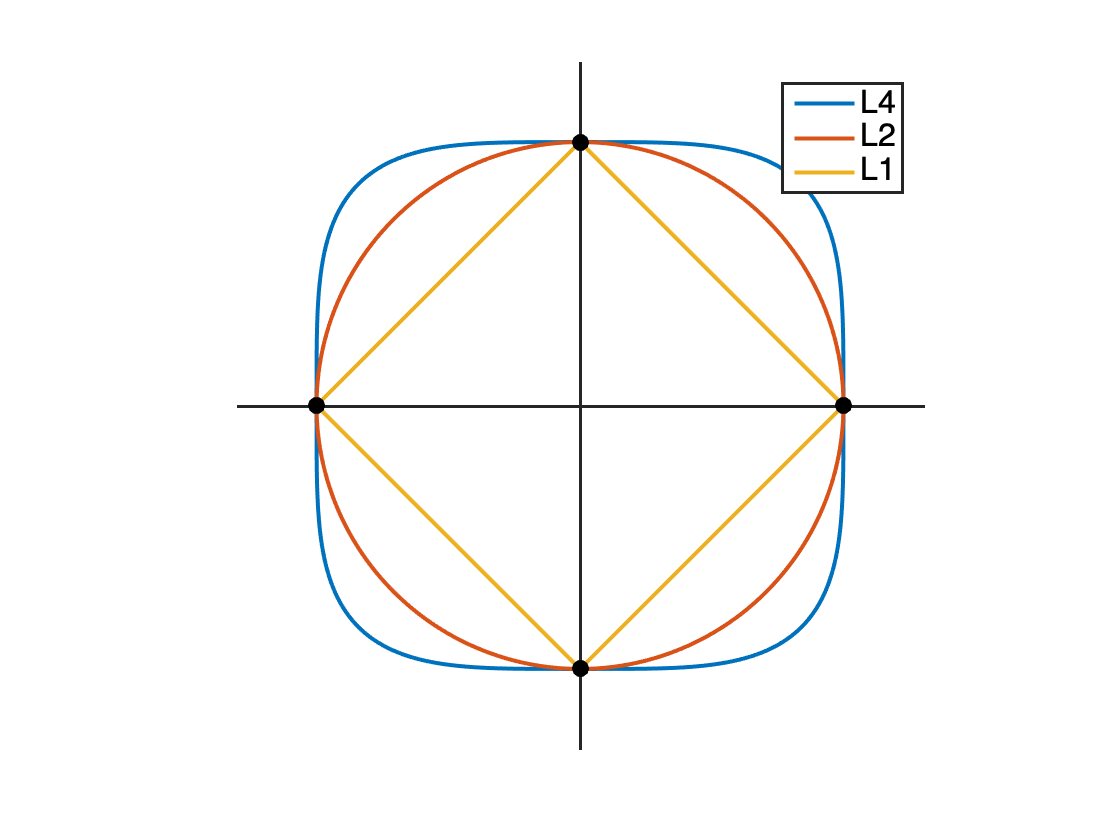
\includegraphics[width=0.6\linewidth]{\toplevelprefix/chapters/chapter2/figs/2DL4Sphere.png}\vspace{-0.1in}
    \caption{Maximizing $\ell^4$ norm or minimizing $\ell^1$ norm promotes sparsity (for vectors on the sphere).}
    \label{fig:L4-sphere}
\end{figure}


\paragraph{Dictionary learning via the MSP algorithm.}

Now suppose that we are given a set of observations:
\begin{equation}
    \x_i = \vU \vz_i + \veps_i,\ \forall i \in [N].
\end{equation}
Let $\vX = [\vx_1, \dots, \vx_N]$ and $\vZ = [\vz_1, \dots, \vz_N]$. The goal is to recover $\vU$ from the data $\vX$. Therefore, given any orthogonal matrix $\vA \in \O(D)$, 
\begin{equation}
    \vA\vx_i = \vA\vU \vz_i + \vA\veps_i
\end{equation}
would be nearly sparse if $\vA = \vU^T$ (as by assumption the noise $\veps_i$ is of small magnitude). 

Also, given $\vU$ is orthogonal and the fact $\veps$ is small, the vector $\vx$ has a predictable expected norm, i.e., $\bE[\norm{\vx}_2^2] \approx \bE[\norm{\vz}_2^2]=d$. It is a known fact that for vectors on a sphere, maximizing the $\ell^4$ norm is equivalent to minimizing the $\ell^0$ norm (for promoting sparsity),
\begin{equation}
    \argmax_{\vz \in \mathbb{S}^n}\|\vz\|_{4}\quad\Leftrightarrow\quad \argmin_{\vz \in \mathbb{S}^n}\|\vz\|_{0}.
\end{equation}
This is illustrated in Figure \ref{fig:L4-sphere}.

An orthogonal matrix $\vA$ preserves the Euclidean (\(\ell^{2}\)) norm: $\|\vA \x\|_2^2 = \|\x\|_2^2$. Therefore, to find the correct orthogonal dictionary $\vU$ from $\vX$, we may try to solve the following optimization program:
\begin{equation}\label{eq0:orthogonal-dictionary-learning-l4}
    \max_{\tilde{\vA} \in \O(D)}\,
     \frac{1}{4} \norm*{
    \tilde{\vA} \vX
    }_4^4 =  \frac{1}{4} \sum_{i=1}^N \norm*{
    \vA \vx_i
    }_4^4
\end{equation}
This is known as the $\ell^4$ maximization problem \cite{Zhai-2020}. After we
find the solution \(\vA^{\star}\), we can take the transpose \(\vU^{\star}
= (\vA^{\star})^{\top}\)
\begin{remark}
    It is also known that for vectors on a sphere, minimizing the $\ell^1$ norm is equivalent to minimizing the $\ell^0$ norm (for promoting sparsity),
\begin{equation*}
            \argmin_{\vz \in \mathbb{S}^n}\|\vz\|_{1}\quad\Leftrightarrow\quad \argmin_{\vz \in \mathbb{S}^n}\|\vz\|_{0},
\end{equation*}
which is also illustrated in Figure \ref{fig:L4-sphere}. This fact can also be exploited to learn the dictionary $\vA$ effectively and efficiently. This was actually explored earlier than the $\ell^4$ norm used here. Interested readers may refer to the work of \cite{qu2020findingsparsestvectorssubspace}.
\end{remark}

Note that the above problem is equivalent to the following constrained optimization problem:
\begin{equation}\label{eq:orthogonal-dictionary-learning-l4}
    \min\,
    -   \frac{1}{4} \norm*{
    \tilde{\vA} \vX
    }_4^4 \quad \mbox{subject to} \quad  \tilde{\vA}^\top\tilde{\vA} = \vI.
\end{equation}
As shown in \cite{Wright-Ma-2022}, using the Lagrange multiplier method, one can derive that the optimal solution to the problem should satisfy the following 
``fixed point'' condition:
\begin{equation}
    \vA^{\star} = \mathcal{P}_{\mathrm O(D)}[( {\vA^{\star} \vX})^{\circ3}\vX^\top],
\end{equation}
where $\mathcal{P}_{\mathrm O(D)}[\,\cdot\,]$ is a projection onto the space of orthogonal matrices $\mathrm O(D)$.\footnote{For any matrix with an SVD: $\vM = \vU\bm \Sigma \vV^\top$, $\mathcal{P}_{\mathrm O(D)}[\vM] = \vU \vV^\top$. We leave this as an exercise for the reader.} 

To compute the fixed point for the above equation, similar to we computed eigenvectors for PCA \eqref{eqn:PCA-fixed-point}, we may take the following power iteration:
\begin{equation}\label{eq:msp_iteration}
    \vA_{t+1} = \mathcal{P}_{\mathrm O(D)}[( {\vA_t \vX})^{\circ3}\vX^\top].
\end{equation}
This is known as the {\em matching, stretching, and projection} (MSP) algorithm proposed by \cite{Zhai-2020}. It was shown that under broad conditions such a greedy algorithm indeed converges to the correct solution at a superlinear rate.

\begin{remark}[Global Optimality of $\ell^4$ Maximization]\label{rem:L4-global}
The constrained $\ell^4$ maximization problem is a nonconvex program. In general one should \textit{not} expect that any greedy (say gradient-descent type) algorithms would converge to the globally optimal solution. Surprisingly, one can show that, unlike general nonconvex programs, the landscape of $\ell^4$ maximization over a sphere
\begin{equation}\label{eq:l4-maximization-sphere}
    \min\,
    -   \frac{1}{4} \norm*{
    \vq^\top \vX
    }_4^4 \quad \mbox{subject to} \quad  \vq^\top\vq = 1.
\end{equation}
is very benign: All local minima are close to the global optima and all critical points are saddle points with a direction of negative curvature. Hence, any descent method with the ability of escaping strict saddle points provably finds global optimal solutions. For more precise statements, interested readers may refer to \cite{Qu2020Geometric}. 
\end{remark}

\begin{remark}[Stable Deep Linear Network]
The above iterative process of computing the dictionary has a natural incremental ``deep learning'' interpretation. Let us define 
$\delta \vA_{t+1} = \vA_{t+1}\vA_{t}^\top$ and $\vZ_t = \vA_t \vX$, then it is easy to show that
$$\delta \vA_{t+1} = \mathcal{P}_{\mathrm O(D)}[(\vZ_t)^{\circ3} \vZ_t^\top].$$ 
If $\vA_t$ converges to the correct dictionary $\vD_o$, then the above iterative encoding process is essentially equivalent to a ``deep linear network'': 
$$\vZ \; \longleftarrow \; \vZ_{t+1} =  \underbrace{\delta \vA_{t+1} \delta \vA_{t} \ldots \delta \vA_{1}}_{\color{red} \text{forward constructed layers}} \vX.$$
Note that the computation of the increment transforms $\delta \vA_{t+1}$ at each layer depends only on the feature output from the previous layer $\vZ_t$. The network is naturally stable as each layer is a norm-preserving orthogonal transform. Despite its resemblance to a linear deep network, backpropagation is unnecessary to learn each layer. All layers are learned in one forward pass!
\end{remark}



% We now derive a fast fixed-point algorithm for this objective by a procedure analogous to what we used to derive FastICA.
% As before, we begin from the first-order optimality condition for optimization over the orthogonal group (Exercise \ref{exercise:orthogonal-group-calculus}), which for the kurtosis maximization objective reads
% \begin{equation}\label{eq:l4-ogrp-fxp-step1}
%     \vX \left( \vX \adj \vU \right)^{\hada 3} = \vU \underbrace{\left. \left(
%     \vU\adj \vX \left( \vX \adj \vU \right)^{\hada 3} 
%     + 
%     \left( \vU\adj \vX \right)^{\hada 3} \vX\adj \vU
%     \right) \right/ 2}_{\vS},
% \end{equation}
% where the value of the symmetric matrix $\vS$ is determined by the constraint that $\vU\adj \vU = \vI$. 
% Next, we recall that that Equation \eqref{eq:l4-ogrp-fxp-step1} is satisfied by \textit{any} critical point of the $\ell^4$ maximization problem, whereas we seek an equation satisfied only by its maximizers.
% In fact, it is possible to show that at any global maximizer $\vU$ to \eqref{eq:orthogonal-dictionary-learning-l4}, the matrix $\vS$ appearing in \eqref{eq:l4-ogrp-fxp-step1} is actually positive semidefinite, i.e.\ $\vS \succeq \mathbf{0}$ (Exercise \ref{exercise:l4-global-maximizers-ogrp}). Using the results of Part 3 of Exercise \ref{exercise:orthogonal-group-calculus} and the singular value decomposition, it is then straightforward
% to show that \textit{normalizing} both sides of \eqref{eq:l4-ogrp-fxp-step1} yields the following fixed point expression, valid at every local maximizer of \eqref{eq:orthogonal-dictionary-learning-l4}:
% \begin{equation}\label{eq:l4-ogrp-fxp}
%     \mathrm{proj}_{\O(d)}\left(
%     \vX \left( \vX \adj \vU \right)^{\hada 3} 
%     \right)
%     = \vU,
% \end{equation}
% where we recall that $\mathrm{proj}_{\O(d)}(\vX) = \vV \vW\adj$, where $\vX = \vV \vS \vW\adj$ is a singular value decomposition of $\vX$ (Part 3 of Exercise \ref{exercise:orthogonal-group-calculus}).
% Iterating the mapping defined by the lefthand side of this fixed point expression then yields the following power method for complete dictionary learning via $\ell^4$ maximization, called the \textit{MSP algorithm} \cite{Zhai2019-oc}:
% \begin{equation}
% \begin{split}\label{eq:msp}
%    \vR^+ &= \vX (\vX\adj \vU)^{\hada 3},  \\
%    \vU^+ &= \vV \vW \adj, \quad \text{where} \enspace \vR^+ = \vV \vS \vW\adj \enspace \textit{is a SVD}.
%    \end{split}
% \end{equation}
% As for the FastICA algorithm seen previously, in practice the MSP algorithm converges extremely rapidly to the true orthogonal dictionary $\vU$ modulo symmetries. 
% %Namely, given the structure of the underlying objective \eqref{eq:orthogonal-dictionary-learning-lasso}, it is only possible to recover $\vU$ up to signed permutations of its rows and columns. 
% %This can be seen as a consequence of our modeling assumptions: either the Bernoulli-Gaussian ICA modeling assumption or the sparsely-used dictionary assumption (c.f.\ Exercise \ref{exercise:symmetry-identifiability}).
% Under idealized conditions, Zhai et al.\ show that the MSP algorithm \eqref{eq:msp} obtains a cubic rate of local convergence, matching the FastICA algorithm's performance \cite{Zhai2019-oc}. 
% %At the same time, it recovers the entire dictionary (or mixing matrix, in the ICA context) in a single round of optimization, while requiring computational operations no more expensive than a singular value decomposition, making it preferable in practice.
% Formulating the dictionary recovery problem in terms of the $\ell^4$ loss, as in the formulation \eqref{eq:orthogonal-dictionary-learning-l4}, additionally has the advantage of conferring robustness to errors and outliers in the data matrix, as Zhai et al.\ show \cite{Zhai-2020}.

% \sdb{Add an algorithm box. Add maybe a numerical experiment.}


%It is important to recognize that this goal cannot always be accomplished: for example, if the independent components $\vz$ are Gaussian, so that $\vz \sim \cN(\Zero, \sigma^2\vI)$,
%we have for any rotation matrix $\vQ$ (so that $\vQ\adj \vQ = \vI$) that $\vQ \vz$ has the same distribution as $\vz$ (Exercise ), meaning that it is impossible to reconstruct $\vz$ from $\vx$ (or $\vU$, for that matter).
%This situation is known as (statistical) non-identifiability; ICA is identifiable only when there is no more than a single Gaussian component. 
%%Even after adding this statistical assumption, note that it is impossible to estimate either the signs or the energies $\Var(z_i)$ of the independent components from $\vx$. 
%%We will therefore assume that each independent component satisfies $\Var(z_i)=1$ for convenience, which makes the independent components identifiable up to their signs \cite{Hyvrinen-2000}.
%These issues can be understood independently of any statistical model for the independent components through the purely geometric notion of \textit{symmetry}, as well: we explore this issue in Exercise \ref{exercise:symmetry-identifiability} below.
%
%
%Contrast the goal of ICA with that of PCA \eqref{eq:pca_model}, where we simply sought to \textit{represent} the data distribution $\vx$ with coefficients $\vz$ such that 
%$\vx \approx \vU \vz$. Geometrically, this corresponds to learning the \textit{subspace} $\mathrm{col}(\vU)$, rather than the specific basis $\vU$ itself.
%In ICA, we are exactly tasked with learning the specific mixing matrix $\vU$, or equivalently the independent components $\vz$.
%It is important to recognize that this goal cannot always be accomplished: for example, if the independent coefficients $\vz$ are Gaussian, so that $\vz \sim \cN(\Zero, \sigma^2\vI)$,
%we have for any rotation matrix $\vQ$ (so that $\vQ\adj \vQ = \vI$) that $\vQ \vz$ has the same distribution as $\vz$ (Exercise \ref{exercise:gaussian-rot-invar}), meaning that it is impossible to reconstruct $\vz$ from $\vx$ (or $\vU$, for that matter).
%We call this situation (statistical) non-identifiability; ICA is identifiable only when there is no more than a single Gaussian component. 
%Even after adding this statistical assumption, note that it is impossible to estimate either the signs or the energies $\Var(z_i)$ of the independent components from $\vx$. 
%We will therefore assume that each independent component satisfies $\Var(z_i)=1$ for convenience, which makes the independent components identifiable up to their signs \cite{Hyvrinen-2000}.
%These issues can be understood independently of any statistical model for the independent components through the purely geometric notion of \textit{symmetry}, as well: we explore this issue in Exercise \ref{exercise:symmetry-identifiability} below.
%
%Given high-dimensional observations $D \geq d$ of non-Gaussian, unit-variance independent components $\vz$,
%we may without loss of generality reduce our study to the case $D = d$ by performing dimensionality reduction using principal component analysis, as we have studied in Section \ref{sub:pca}. Moreover, by a `whitening' transformation of the data (Exercise \ref{exercise:whitening}), we may assume without loss of generality that $\vU\adj \vU = \vI$, i.e.\ that $\vU$ is an orthogonal matrix.
%



\subsection{Connection to ICA and Kurtosis}
With the Bernoulli-Gaussian model, the variables $z_i$'s are independent and non-Gaussian. Then, there is a clear correspondence between the dictionary learning and the classic independent component analysis (ICA), to the extent that algorithms to solve one problem can be used to solve the other.\footnote{We explore this issue in more depth in Exercise \ref{exercise:symmetry-identifiability}, where a connection between non-Gaussianity of the independent components and the purely geometric notion of symmetry is made. This issue is related to our observation above that PCA does not work for recovering sparsely-used orthogonal dictionaries: in the statistical setting, it can be related to rotational invariance of the Gaussian distribution (Exercise \ref{exercise:gaussian-rot-invar}).} 
%\sdb{add a figure of BG model / subspaces picture}    


Towards deriving an algorithm based on ICA, we focus on an objective function known as \textit{kurtosis}, which is used in ICA as a direct consequence of the non-Gaussianity of the components. The \textit{kurtosis}, or fourth-order cumulant, of a zero-mean random variable $X$ is defined as
\begin{equation}\label{eq:kurtosis}
\kurt(X) = \Ex{X^4} - 3 (\Ex{X^2})^2.
\end{equation}
If we have only finite samples from the random variable $X$ arranged into a vector $\vx = [x_1, \dots, x_N]$, we define kurtosis through their empirical average, which yields
\begin{equation}\label{eq:kurtosis-vector}
\kurt(\vx) = \frac{1}{N} \norm{\vx}_4^4 - \frac{3}{N^2} \norm{\vx}_2^4.
\end{equation}
Finally, for random vectors, we define their kurtosis as the sum of each component's scalar kurtosis.
Kurtosis is a natural loss function for ICA because for Gaussian $X$, kurtosis is zero; the reader can verify further that the Bernoulli-Gaussian distribution has positive kurtosis. 
%\sdb{Could we recast kurtosis objective more quickly as $\ell^4$ and the connection to sparsity (duality) via noting that normalization makes the $\ell^4$ term the relevant one...? This can become more unified (low-dimensionality vs.\ non-gaussianity...)}
Thus a natural procedure for seeking non-Gaussian independent components is to search for a set of mutually-orthogonal directions $\vV \in \R^{d \times k}$ such that $\vV^\top \vX$ has maximal kurtosis, where $\vX = \vU \vZ \in \R^{D \times N}$ is the Bernoulli-Gaussian ICA data matrix.
%In general, kurtosis measures the prevalence of outliers (or `atypical' values) in a distribution: distributions with a higher prevalence of outliers have positive kurtosis, and those that do not have negative kurtosis.\footnote{For example, the Laplace distribution, which is proportional to $\exp(-\norm{\vx}_1)$, has positive kurtosis; the uniform distribution on $[-1, 1]$ has negative kurtosis.}
%\sdb{A figure here.}.
Formally, we seek to solve the problem
\begin{equation}
    \max_{\vV^\top \vV = \vI} \kurt(\vV^\top \vX).
\end{equation}
At one extreme, we may set $k = D$ and seek to recover the entire dictionary $\vU$ in a single shot.  At the other extreme, we may set $k=1$ and seek to recover a single direction (column of $\vU$) at a time, performing \textit{deflation}, i.e., replacing the data matrix $\vX$ by $(\vI - \vu\vu^\top) \vX$, after each step before finding another direction.
There is a natural tradeoff between the scalability of the $k=1$ incremental approach and the efficiency and robustness of the $k=D$ approach. We will therefore consider both below.

\paragraph{Incremental ICA: correctness and FastICA algorithm.}
The FastICA algorithm, advanced by Hyv\"{a}rinen and Oja \cite{hyvarinen-1997}, is a fast fixed-point algorithm for solving the $k=1$ kurtosis maximization scheme for ICA.
The problem at hand is
\begin{equation}\label{eq:kurtosis-maximization-sphere-finitesample}
    \max_{\norm{\vv}_2^2 = 1}\, \kurt(\vX^\top \vv).
\end{equation}
First, we will perform some very basic analysis of this objective to verify its correctness. Notice by the change of variables $\vw = \vU^\top \vv$ that this problem is equivalent to
\begin{equation*}
    \max_{\norm{\vw}_2^2 = 1}\, 
    \mathrm{kurt}(\vZ^\top \vw).
\end{equation*}
This objective is simple enough that we can make strong statements about its correctness as a formulation for recovering the dictionary $\vU$.
For example, in the population setting where $N \to \infty$, 
we may use additivity properties of the kurtosis (Exercise \ref{exercise:kurtosis-linearity-properties}) and our assumed normalization on the independent components to write the previous problem equivalently as
\begin{equation}\label{eq:kurtosis-maximization-sphere-population-simple}
    \max_{\norm{\vw}_2^2 = 1}\, 
    \sum_{i=1}^d \mathrm{kurt}(z_i) w_i^4.
\end{equation}
It can be shown that under the Bernoulli-Gaussian assumption, the optimization landscape of this problem is ``benign'' (Exercise \ref{exercise:kurtosis-sphere-landscape})---meaning that all local maxima of the objective function correspond to the recovery of one of the independent components.
One efficient and scalable way to compute one of these maxima is via first-order optimization algorithms, which iteratively follow the gradient of the objective function and project onto the constraint set $\set{\vw \given \norm{\vw}_2^2 = 1}$.
Since we have assumed that each $z_i$ satisfies $\Var(z_i)=1$, we 
have for large $N$
\begin{equation}\label{eq:kurtosis-approximation-l4}
    \kurt(\vX^\top \vu)
    \approx
    \tfrac{1}{N} \norm{\vX^\top \vu}_4^4 - 3 \norm{\vu}_2^4.
\end{equation}
We can then derive a corresponding approximation to the gradient:
\begin{equation*}
    \nabla_{\vu} \kurt(\vX^\top \vu)
    \approx
    \tfrac{4}{N} \vX (\vX^\top \vu)^{\hada 3}
    - 12 \norm{\vu}_2^2 \vu.
\end{equation*}
The FastICA algorithm uses a fixed-point method to compute directions of maximum kurtosis. It starts from the first-order optimality conditions for the kurtosis maximization problem, given the preceding gradient approximation and the constraint set, which read
\begin{align}\label{eq:kurtosis-max-sphere-stationarity}
   %\vP_{\vu}^\perp\left( 
   %\frac{1}{N}\vX (\vX\adj \vu)^{\hada 3} - 3 \norm{\vu}_2^2 \vu
   %\right) = \Zero
   %\iff
   \vX (\vX^\top \vu)^{\hada 3} 
   = 
   \underbrace{
   \ip*{\vu}{
   \vX (\vX^\top \vu)^{\hada 3} 
   }}_{\lambda} \vu,
   %\lambda \vu,
\end{align}
where the specific value of $\lambda$ is determined using the unit norm constraint on $\vu$.
Exercise \ref{exercise:sphere-calculus} describes the mathematical background necessary to derive these optimality conditions from first principles.
Equation \eqref{eq:kurtosis-max-sphere-stationarity} is satisfied by \textit{any} critical point of the kurtosis maximization problem; we want to derive an equation satisfied by only the maximizers.
After noticing that $\lambda = \norm{\vX^\top \vu}_4^4$, we equivalently re-express \eqref{eq:kurtosis-max-sphere-stationarity} as the modified equation
\begin{align}\label{eq:kurtosis-max-sphere-stationarity-modified}
   \frac{1}{N}\vX (\vX^\top \vu)^{\hada 3} 
   - 
   3 \vu
   = 
   \left(
   \frac{\lambda}{N} - 3
   \right)
   \vu,
\end{align}
and realize that any maximizer of \eqref{eq:kurtosis-maximization-sphere-finitesample} 
must satisfy $\lambda / N - 3 > 0$,
assuming that $N$ is sufficiently large.
Hence, we may \textit{normalize} both sides of \eqref{eq:kurtosis-max-sphere-stationarity-modified},
giving the following fixed-point equation satisfied by every maximizer of \eqref{eq:kurtosis-maximization-sphere-finitesample}:
\begin{align}\label{eq:kurtosis-max-sphere-fxp}
\frac{
   \frac{1}{N}\vX (\vX^\top \vu)^{\hada 3} 
   - 
   3 \vu
   }{
   \norm*{
   \frac{1}{N}\vX (\vX^\top \vu)^{\hada 3} 
   - 
   3 \vu
   }_2
   }
   =
   \vu.
\end{align}
Iterating the mapping defined by the lefthand side of this fixed point expression then yields the FastICA algorithm of Hyv\"{a}rinen and Oja \cite{hyvarinen-1997}:
\begin{equation}
\begin{split}\label{eq:fast-ica}
   \vv^+ &= \tfrac{1}{N}\vX (\vX^\top \vu)^{\hada 3}- 3 \vu
   ,  \\
   \vu^+ &= \vv^+ / \norm*{\vv^+}_2.
   \end{split}
\end{equation}
It turns out that the FastICA algorithm converges extremely rapidly (actually at a \textit{cubic} rate) to columns of the dictionary $\vU$. 
Exercise \ref{exercise:fast-ica-convergence} explores these issues in more depth. \DP{referenced exercise isn't complete yet} %\yima{Missing reference to exercise.}
Comparing the FastICA algorithm \eqref{eq:fast-ica} to the power method studied in \ref{sub:pca} for the PCA problem, we notice a striking similarity. Indeed, FastICA is essentially a modified power method, involving the gradient of the empirical kurtosis rather than the simpler linear gradient of the PCA objective.

%\sdb{Add an algorithm box for FastICA.}






%\subsection{Solving ICA by Optimizing Kurtosis with Gradient Ascent}\label{sec:ica-via-kurtosis-gd}
%
%We have seen that non-Gaussianity of the independent components $\vz$ is an essential assumption for the ICA problem to be tractable.
%We can exploit this insight further to develop computationally-efficient algorithms for ICA. 
%The \textit{kurtosis}, or fourth-order cumulant, of a zero-mean random variable $X$ is defined as
%\begin{equation}\label{eq:kurtosis}
%\kurt(X) = \Ex{X^4} - 3 (\Ex{X^2})^2.
%\end{equation}
%If we have only finite samples from the random variable $X$ arranged into a vector $\vx = [x_1, \dots, x_N]$, we define kurtosis through their empirical average, which yields
%\begin{equation}\label{eq:kurtosis-vector}
%\kurt(\vx) = \tfrac{1}{N} \norm{\vx}_4^4 - \tfrac{3}{N^2} \norm{\vx}_2^4.
%\end{equation}
%If $X$ is Gaussian, its kurtosis is zero. In general, kurtosis measures the prevalence of outliers (or `atypical' values) in a distribution: distributions with a higher prevalence of outliers have positive kurtosis, and those that do not have negative kurtosis.\footnote{For example, the Laplace distribution, which is proportional to $\exp(-\norm{\vx}_1)$, has positive kurtosis; the uniform distribution on $[-1, 1]$ has negative kurtosis.}
%\sdb{A figure here.}.
%It can therefore be used in an attempt to ``pick out'' independent non-Gaussian components from the observation $\vx$, by the following procedure: 
%\begin{enumerate}
%    \item Using the observed data $\vX = [\vx_1, \dots, \vx_N]$, find a direction $\vu \in \R^d$ with unit norm such that $\vX\adj\vu$ has maximum or minimum kurtosis.
%    \item Perform \textit{deflation}: with the found direction $\vu$, remove $\vu$ from the column space of $\vX$ to continue searching for new directions, via $\vX^+ = (\vI - \vu\vu\adj) \vX$.
%    \item Repeat the previous two steps until all independent components have been recovered.
%\end{enumerate}
%This ``greedy'' approach, which incrementally finds one independent component at a time, is one of the oldest algorithms in the ICA literature, and parallels the use of such greedy algorithms in many other areas of signal processing and machine learning---from the PCA problem we saw in Section \ref{sub:pca}, to algorithms for signal recovery such as orthogonal matching pursuit, and optimization algorithms such as Frank-Wolfe methods \sdb{add refs}.
%It splits the ICA problem into multiple simple subproblems, each of which is straightforward to solve. 
%However, it can lead to long runtimes, and \textit{a priori} may fail due to compounding errors if subproblems are solved inaccurately. 
%We will see how to correct these deficiencies later, at least in a special case of the general ICA problem.
%%\sdb{Can we do some ``history'' here---from one at a time, to ``global and cut'' (all at once, + model selection)...}
%
%For now, let us work out the first step of the above greedy procedure for ICA in detail, in the ``population'' case where $N \to \infty$. The optimization problem at hand reads
%\begin{equation}\label{eq:kurtosis-maximization-sphere}
%    \max_{\norm{\vu}_2^2 = 1}\, 
%    \kurt(\ip{\vx}{\vu}).
%\end{equation}
%Notice by the change of variables $\vw = \vU\adj \vu$ that this problem is equivalent to
%\begin{equation*}
%    \max_{\norm{\vw}_2^2 = 1}\, 
%    \mathrm{kurt}(\ip{\vz}{\vw}).
%\end{equation*}
%Using additivity properties of the kurtosis (Exercise \ref{exercise:kurtosis-linearity-properties}), we find that this problem can be written as
%\begin{equation}\label{eq:kurtosis-maximization-sphere-population-simple}
%    \max_{\norm{\vw}_2^2 = 1}\, 
%    \sum_{i=1}^d \mathrm{kurt}(z_i) w_i^4.
%\end{equation}
%It can be shown that whenever there is at least one component with positive kurtosis, the optimization landscape of this problem is ``benign'' (Exercise \ref{exercise:kurtosis-sphere-landscape})---meaning that all local maxima of the objective function correspond to the recovery of one of the independent components.
%Moreover, whenever no independent components have zero kurtosis, natural optimization algorithms such as gradient descent with a small amount of added noise provably converge to these local maxima in polynomial time \cite{Jin2017-zt}.
%In fact, the kurtosis maximization problem \eqref{eq:kurtosis-maximization-sphere-population-simple} has even more structure that allows gradient descent \textit{with no added noise} to rapidly converge to maximizers under slightly stronger assumptions on the independent components \cite{Gilboa2019-px}.
%These technical analyses are out of the scope of our current discussion---we only mention them as an assurance that 
%the scalable and efficient optimization methods we are developing for the ICA problem are in fact guaranteed to succeed.
%
%Now, the finite-sample version of \eqref{eq:kurtosis-maximization-sphere} reads as
%\begin{equation}\label{eq:kurtosis-maximization-sphere-finitesample}
%    \max_{\norm{\vu}_2^2 = 1}\, 
%    \kurt(\vX\adj \vu).
%\end{equation}
%Since we have assumed that each $z_i$ satisfies $\Var(z_i)=1$, we 
%have for large $N$
%\begin{equation}\label{eq:kurtosis-approximation-l4}
%    \kurt(\vX\adj \vu)
%    \approx
%    \tfrac{1}{N} \norm{\vX\adj \vu}_4^4 - 3 \norm{\vu}_2^4.
%\end{equation}
%We can then derive a corresponding approximation to the gradient:
%\begin{equation*}
%    \nabla_{\vu} \kurt(\vX\adj \vu)
%    \approx
%    \tfrac{4}{N} \vX (\vX\adj \vu)^{\hada 3}
%    - 12 \norm{\vu}_2^2 \vu.
%\end{equation*}
%Here, $\va^{\hada 3}$ denotes the vector $\va$ with each element raised to the third power.
%The final detail to account for is solving the problem \eqref{eq:kurtosis-maximization-sphere-finitesample} not over the ambient space $\vu \in \R^d$, but over the constraint set $\set{\vu \in \R^d \given \norm{\vu}_2^2 = 1}$.
%For a gradient descent-based solver for \eqref{eq:kurtosis-maximization-sphere-finitesample}, there are two places where this detail must be accounted for: (\sdb{could make a figure for this if relevant enough...})
%\begin{enumerate}
%    \item \textbf{Search direction:} A gradient ascent algorithm on $\R^d$ follows a scaled multiple of the Euclidean gradient to update the current iterate: that is, the search direction is $\eta \nabla_{\vu} \kurt(\vX\adj \vu)$, for a ``step size'' $\eta > 0$.
%    To account for the constraint set $\set{\vu \in \R^d \given \norm{\vu}_2^2 = 1}$, one follows not the gradient itself, but its projection into a subspace representing only those directions at the point $\vu \in \set{\vu \in \R^d \given \norm{\vu}_2^2 = 1}$ which are (locally) parallel to the constraint set.
%    It turns out that for this spherical constraint set, this implies the search direction
%    \begin{equation}\label{eq:kurtosis-maximization-sphere-search-dir}
%        \eta \vP_{\vu}^\perp \nabla_{\vu} \kurt(\vX\adj \vu),
%    \end{equation}
%    where $\vP_{\vu}^\perp = \vI - \vu\vu\adj$ is the orthogonal projection onto the orthogonal complement of the subspace $\Span(\set{\vu})$ (Exercise \ref{exercise:sphere-calculus}).
%    \item \textbf{Iterate feasibility:} After following the search direction, an extra step must be taken to ensure that the updated iterate stays within the constraint set. This can be accomplished with projected gradient ascent: one simply projects the result of following the search direction onto the constraint set. For the spherical constraint set, 
%    this projection is given by dividing by the $\ell^2$ norm of the input:
%    \begin{equation*}
%        \mathrm{proj}_{\mathbb{S}^{d-1}}\left( \vv \right)
%        = \frac{\vv}{\norm{\vv}_2}.
%    \end{equation*}
%\end{enumerate}
%Thus, we obtain the following gradient ascent algorithm for solving \eqref{eq:kurtosis-maximization-sphere-finitesample}: 
%\begin{equation}
%\begin{split}\label{eq:kurtosis-maximization-gradient-ascent}
%   \vv^+ &= \vu + \tfrac{4\eta}{N} %\left( 
%    \vP_{\vu}^\perp \vX (\vX\adj \vu)^{\hada 3}, \\
%    %- 12 \vu % \norm{\vw}_2^2 \vw
%   %\right),  \\
%   \vu^+ &= \mathrm{proj}_{\mathbb{S}^{d-1}}\left( \vv^+ \right) = \vv^+ / \norm*{\vv^+}_2.
%   \end{split}
%\end{equation}
%Here, $\eta > 0$ is the step size, which can vary between iterations if desired.
%We thus obtain our first computationally-efficient solution to the ICA problem.


%\subsection{Optimizing Kurtosis with the Power Method (FastICA)}
%Gradient-based algorithms for optimizing differentiable objective functions like our iteration \eqref{eq:kurtosis-maximization-gradient-ascent} for solving the ICA problem typically converge no faster than the rate $O(1/k)$ in the worst case, where $k$ is the iteration number. 
%Near a maximizer, such gradient ascent algorithms often obtain more rapid \textit{linear convergence}, i.e.\ worst-case rates $O(c^{k})$, where $0 < c < 1$ is called the rate of (linear) convergence.
%However, in highly structured signal recovery problems like ICA where local optima correspond to low-dimensional distributions (in particular, specific columns of the mixing matrix $\vU$), 
%it is possible to develop algorithms that converge \textit{globally} at superlinear rates under mild assumptions on the data.
%We have already seen one such example of a method in Section \ref{sub:pca}, namely the \textit{power method} for principal component analysis. 
%In fact, the parallel structure of the kurtosis maximization problem for ICA \eqref{eq:kurtosis-maximization-sphere-population-simple} enables the derivation of a power method for kurtosis maximization, as well, which we will now take up.
%This derivation will lead us to an algorithm originally proposed by Hyv\"{a}rinen and Oja, called FastICA
%\cite{hyvarinen-1997}.
%
%The key to this derivation is to reconsider the gradient ascent update, which follows the search
%direction \eqref{eq:kurtosis-maximization-sphere-search-dir}, from a fixed-point perspective.
%In this view, we will express the first-order optimality conditions for the problem \eqref{eq:kurtosis-maximization-sphere-finitesample} in a form that allows us to derive
%a fixed-point equation that every maximizer of \eqref{eq:kurtosis-maximization-sphere-finitesample} must satisfy.
%Then we will obtain an algorithm for solving this fixed-point equation by the standard approach of repeatedly iterating the mapping.
%In the present setting, one begins by looking at the first-order stationarity condition
%\begin{align}\label{eq:kurtosis-max-sphere-stationarity}
%   \vP_{\vu}^\perp\left( 
%   \frac{1}{N}\vX (\vX\adj \vu)^{\hada 3} - 3 \norm{\vu}_2^2 \vu
%   \right) = \Zero
%   \iff
%   \vX (\vX\adj \vu)^{\hada 3} 
%   = 
%   \underbrace{
%   \ip*{\vu}{
%   \vX (\vX\adj \vu)^{\hada 3} 
%   }}_{\lambda} \vu,
%   %\lambda \vu,
%\end{align}
%where the specific value of $\lambda$ is determined using the unit norm constraint on $\vu$.
%Equation \eqref{eq:kurtosis-max-sphere-stationarity} is satisfied by \textit{any} critical point of the kurtosis maximization problem; we want to derive an equation satisfied by only the maximizers.
%After noticing that $\lambda = \norm{\vX\adj \vu}_4^4$, we equivalently re-express \eqref{eq:kurtosis-max-sphere-stationarity} as the modified equation
%\begin{align}\label{eq:kurtosis-max-sphere-stationarity-modified}
%   \frac{1}{N}\vX (\vX\adj \vu)^{\hada 3} 
%   - 
%   3 \vu
%   = 
%   \left(
%   \frac{\lambda}{N} - 3
%   \right)
%   \vu,
%\end{align}
%and realize that any maximizer of \eqref{eq:kurtosis-maximization-sphere-finitesample} 
%must satisfy $\lambda / N - 3 > 0$
%(assuming that $N$ is sufficiently large and that $\kurt(z_i) > 0$ for at least one $i$, making the problem nontrivial).
%Hence, we may \textit{normalize} both sides of \eqref{eq:kurtosis-max-sphere-stationarity-modified},
%giving the following fixed-point equation satisfied by every maximizer of \eqref{eq:kurtosis-maximization-sphere-finitesample}:
%\begin{align}\label{eq:kurtosis-max-sphere-fxp}
%\frac{
%   \frac{1}{N}\vX (\vX\adj \vu)^{\hada 3} 
%   - 
%   3 \vu
%   }{
%   \norm*{
%   \frac{1}{N}\vX (\vX\adj \vu)^{\hada 3} 
%   - 
%   3 \vu
%   }_2
%   }
%   =
%   \vu.
%\end{align}
%Iterating the mapping defined by the lefthand side of this fixed point expression then yields the FastICA algorithm of Hyv\"{a}rinen and Oja \cite{hyvarinen-1997}:
%\begin{equation}
%\begin{split}\label{eq:fast-ica}
%   \vv^+ &= \tfrac{1}{N}\vX (\vX\adj \vu)^{\hada 3}- 3 \vu
%   ,  \\
%   \vu^+ &= \vv^+ / \norm*{\vv^+}_2.
%   \end{split}
%\end{equation}
%Although our derivation hinges on the \textit{necessity} of the fixed point condition \eqref{eq:kurtosis-max-sphere-fxp} for a point $\vu$ to be a maximizer of the kurtosis maximization problem, rather than its sufficiency, it turns out that the FastICA algorithm indeed converges extremely rapidly (actually at a super-linear \textit{cubic} rate) to desirable solutions, namely columns of the mixing matrix $\vU$. 
%The only caveat to mention is that it does not necessarily converge to the solution of the problem \eqref{eq:kurtosis-maximization-sphere-finitesample}: under suitable assumptions, it will converge to the column of $\vU$ associated to the independent component $z_i$ with the largest absolute value of its kurtosis, which in the setting of ICA is an acceptable result.
%Exercise \ref{exercise:fast-ica-convergence} explores these issues in more depth.
%
%Comparing the FastICA algorithm \eqref{eq:fast-ica} to the power method studied in \ref{sub:pca} for the PCA problem, we notice a striking similarity. Indeed, FastICA is essentially a modified power method, involving the gradient of the empirical kurtosis rather than the simpler linear gradient of the PCA objective.
%%This is an example of a \textit{power method} for the single-component kurtosis maximization problem \eqref{eq:kurtosis-maximization-sphere-finitesample}.
%We will see more examples of the utility and applicability of this family of algorithms for rapidly converging to low-dimensional structures soon.

%\sdb{Could be possible to write about other approaches to ICA? possible connections to maximum MI (could tie in elsewhere, e.g., the next chapter / compression?)}

%\subsection{Complete Dictionary Learning}
%
%To understand the geometric significance of the ICA problem more deeply, and in particular its role as a generalization of the single-low-rank-subspace PCA model, it is helpful to focus
%on a specific statistical model of interest for the independent components $\vz$. 
%Here, we assume each independent component is distributed as $\mathrm{Bern}(\theta) \cdot \cN(0, 1/\theta)$: that is, the product of a Bernoulli random variable with probability $\theta$ of being $1$ and $1-\theta$ of being $0$, and an independent Gaussian random variable with variance $1/\theta$. The normalization is chosen so that $\Var(z_i) = 1$, and hence $\bE[\norm{\vz}_2^2]=d$. Using independence and the fact that the fourth moment of the standard Gaussian is $3$, one calculates $\kurt(z_i) = 3\theta(1-\theta) > 0$, so this model is indeed amenable to ICA.
%
%Notice that this modeling assumption implies that the vector of independent components $\vz$ is typically \textit{very sparse}, i.e.\ having a small number of nonzero entries (Figure \ref{} \sdb{add a figure of BG model / subspaces picture}).
%We measure the sparsity of a vector through its so-called $\ell^0$ norm, which counts the number of nonzero entries of the vector:
%It is easy to calculate $\bE\left[\norm{\vz}_0\right] = d\theta$, so that when the Bernoulli
%rate parameter $\theta$ is chosen to be inversely proportional to $d$, the vector of independent components $\vz$ is indeed typically very sparse \sdb{It might feel a bit weird that to get $\vz$ to be sparse, you need to pick e.g.\ $\theta = 2/d$, which means the variance of each entry's associated Gaussian is $d/2$ (very large). This is because of the insistence on normalizing so that $\Var(z_i) = 1$. I think this insistence makes sense given the derivations it helps with throughout this section. But it's worth noting and reflecting on (let me know what you think).}.
%Because each component of $\vz$ is \textit{independent}, the realizations of the observation $\vx$ therefore correspond to linear combinations of a small number of columns of the mixing matrix $\vU$. This means the observations are drawn from a \textit{mixture of subspaces}, parameterized by (typically) all possible choices of at most $\bE\left[\norm{\vz}_0\right]$ columns of $\vU$ (Figure \ref{} \sdb{add figure; two panel previous...}).
%
%This geometric perspective corresponds to a highly related family of models and problems called \textit{dictionary learning}. Here, the observations $\vx$ are viewed as sparse linear combinations of a small number of ``atoms'' (columns) of a ``dictionary'' namely the matrix $\vU$. 
%The goal is identical to the ICA problem \eqref{eq:ica-model-ch2}, but algorithms for solving the dictionary learning problem exploit the underlying geometric assumption that the vector $\vz$ is sparse, rather than the independence of its components as in ICA.
%In the present setting, where the dictionary $\vU$ is an orthogonal matrix (or more generally, a full-rank square matrix), the specific recovery problem is called \textit{complete dictionary learning}.
%The case where $d > D$ is called \textit{overcomplete} dictionary learning---we will study it in the next section.
%The dictionary learning model was originally motivated as a biologically-plausible algorithm for early vision, based on experiments in the visual cortex by Olshausen and Field \cite{OlshausenB1996} (Figure \ref{fig:} \sdb{add ...}). It was later shown to imply competitive analytical algorithms for a variety of applied problems, including image denoising \cite{Aharon2006-ki} \sdb{add more}, with strong theoretical guarantees \cite{Spielman2012-tl} \sdb{add more, think about citing TCS people}.
%
%A typical algorithm for orthogonal dictionary learning involves the minimization of a regularized loss that follows a fundamental principle for signal recovery: \textit{we seek the most structured signals that are consistent with our observations}. In the context of dictionary learning, where we have reason to assume that the vector $\vz$ is sparse, this corresponds to an objective function of the form
%\begin{equation}\label{eq:orthogonal-dictionary-learning-lasso}
%    \min_{\vU \in \mathrm{O}(d), \vZ \in \R^{d \times N}}\,
%    \frac{1}{2} \norm*{ \vU \vZ - \vX}_2^2 + \lambda \norm{\vZ}_1,
%\end{equation}
%where $\norm{\vZ}_1 = \sum_{i, j} \abs{Z_{ij}}$ is the $\ell^1$ norm, a tractable surrogate for the sparsity-measuring $\ell^0$ norm, and the parameter $\lambda > 0$ is tuned to balance between the consistency and structure-enforcing behavior of the loss.
%Compared to the ICA formulations derived in the previous section, which in the dictionary learning context correspond to the recovery of only a single column of the mixing matrix $\vU$ at a time, 
%the formulation \eqref{eq:orthogonal-dictionary-learning-lasso} seeks to recover the entire dictionary in one shot of optimization by optimizing over the set of orthogonal matrices, rather than the sphere, as in \eqref{eq:kurtosis-maximization-sphere-finitesample}.
%This confers additional robustness in the form of avoiding issues due to inexact solutions of subproblems in the deflation method we derived previously. We will show soon that the complexity of optimizing over this more complex constraint set can be dealt with in a manner very similar to our 
%work for the case of the sphere.
%Now, given that $\vU$ is orthogonal, it is possible to simplify the problem \eqref{eq:orthogonal-dictionary-learning-lasso} to the equivalent form 
%\begin{equation}\label{eq:orthogonal-dictionary-learning-lasso-simplified}
%    \min_{\vU \in \mathrm{O}(d)}\,
%    \sum_{i, j} g_{\lambda}\left(
%    \ip{\vu_i}{\vx_j}
%    \right),
%\end{equation}
%where $g_{\lambda} : \R \to \R$ is a certain scalar function, called the \textit{Huber loss}, which promotes sparsity (Exercise \ref{exercise:orthogonal-dl-simplifying}).
%This objective has a striking similarity to the kurtosis maximization objective \eqref{eq:kurtosis-maximization-sphere-finitesample}, generalized to an orthogonal matrix decision variable rather than a single column of this matrix.
%Both objectives consist of an elementwise loss over the dictionary-data product $\vX\adj \vU$, but for the kurtosis loss we \textit{maximize} the objective, and for the sparsifying objective \eqref{eq:orthogonal-dictionary-learning-lasso-simplified} we \textit{minimize}. 
%These two approaches are indeed equivalent: we see in the analysis of the kurtosis maximization problem's landscape in Exercise \ref{exercise:kurtosis-sphere-landscape} that the optimizers of this maximization objective correspond to \textit{sparse vectors}, just as \eqref{eq:orthogonal-dictionary-learning-lasso-simplified} explicitly promotes the sparsity of the solution.
%
%Motivated by this equivalence, we may consider a simple alternative to the sparsity-promoting formulation \eqref{eq:orthogonal-dictionary-learning-lasso-simplified}, involving instead the kurtosis:
%\begin{equation}\label{eq:orthogonal-dictionary-learning-kurtosis}
%    \max_{\vU \in \mathrm{O}(d)}\,
%    \sum_{i=1}^d \kurt\left(
%    \vX\adj \vu_i
%    \right).
%\end{equation}
%Given our normalization assumption enforcing $\Var(z_i) = 1$, we can simplify the kurtosis once again with the approximation \eqref{eq:kurtosis-approximation-l4} to obtain the so-called \textit{$\ell^4$ maximization} objective for orthogonal dictionary learning, which has been extensively practiced in recent years \cite{Zhai2019-oc}:
%\begin{equation}\label{eq:orthogonal-dictionary-learning-l4}
%    \max_{\vU \in \mathrm{O}(d)}\,
%    \sum_{i=1}^d \norm*{
%    \vX\adj \vu_i
%    }_4^4.
%\end{equation}
%We will now derive an efficient and scalable algorithm for orthogonal dictionary learning via the objective \eqref{eq:orthogonal-dictionary-learning-l4}. 
%We follow the fixed point approach advanced in the previous section, which there led us to the FastICA algorithm.
%In this case, it will lead us to a power method for the objective \eqref{eq:orthogonal-dictionary-learning-l4}, which has been dubbed the ``MSP algorithm'' (matching, stretching, and projection) by Zhai et al.\ \cite{Zhai2019-oc}.
%As before, we begin from the first-order optimality condition for optimization over the orthogonal group (Exercise \ref{exercise:orthogonal-group-calculus}), which in our case reads
%\begin{equation}\label{eq:l4-ogrp-fxp-step1}
%    \vX \left( \vX \adj \vU \right)^{\hada 3} = \vU \underbrace{\left. \left(
%    \vU\adj \vX \left( \vX \adj \vU \right)^{\hada 3} 
%    + 
%    \left( \vU\adj \vX \right)^{\hada 3} \vX\adj \vU
%    \right) \right/ 2}_{\vS},
%\end{equation}
%where the value of the symmetric matrix $\vS$ is determined by the constraint that $\vU\adj \vU = \vI$. 
%Next, we recall that that Equation \eqref{eq:l4-ogrp-fxp-step1} is satisfied by \textit{any} critical point of the $\ell^4$ maximization problem, whereas we seek an equation satisfied only by its maximizers.
%In fact, it is possible to show that at any maximizer $\vU$ to \eqref{eq:orthogonal-dictionary-learning-l4}, the matrix $\vS$ appearing in \eqref{eq:l4-ogrp-fxp-step1} is actually positive semidefinite, i.e.\ $\vS \succeq \mathbf{0}$ (Exercise \ref{exercise:l4-maximizers-ogrp}). Using the results of Part 3 of Exercise \ref{exercise:orthogonal-group-calculus} and the singular value decomposition, it is then straightforward
%to show that \textit{normalizing} both sides of \eqref{eq:l4-ogrp-fxp-step1} yields the following fixed point expression, valid at every local maximizer of \eqref{eq:orthogonal-dictionary-learning-l4}:
%\begin{equation}\label{eq:l4-ogrp-fxp}
%    \mathrm{proj}_{\O(d)}\left(
%    \vX \left( \vX \adj \vU \right)^{\hada 3} 
%    \right)
%    = \vU,
%\end{equation}
%where we recall that $\mathrm{proj}_{\O(d)}(\vX) = \vV \vW\adj$, where $\vX = \vV \vS \vW\adj$ is a singular value decomposition of $\vX$ (Part 3 of Exercise \ref{exercise:orthogonal-group-calculus}).
%Iterating the mapping defined by the lefthand side of this fixed point expression then yields the following power method for complete dictionary learning via $\ell^4$ maximization, called the \textit{MSP algorithm} \cite{Zhai2019-oc}:
%\begin{equation}
%\begin{split}\label{eq:msp}
%   \vR^+ &= \vX (\vX\adj \vU)^{\hada 3},  \\
%   \vU^+ &= \vV \vW \adj, \quad \text{where} \enspace \vR^+ = \vV \vS \vW\adj \enspace \textit{is a SVD}.
%   \end{split}
%\end{equation}
%As for the FastICA algorithm seen previously, in practice the MSP algorithm converges extremely rapidly to the true orthogonal dictionary $\vU$ modulo symmetries. Namely, given the structure of the underlying objective \eqref{eq:orthogonal-dictionary-learning-lasso}, it is only possible to recover $\vU$ up to signed permutations of its rows and columns. 
%This can be seen as a consequence of our modeling assumptions: either the Bernoulli-Gaussian ICA modeling assumption or the sparsely-used dictionary assumption (c.f.\ Exercise \ref{exercise:symmetry-identifiability}).
%Under idealized conditions, Zhai et al.\ show that the MSP algorithm \eqref{eq:msp} obtains a cubic rate of local convergence, matching the FastICA algorithm's performance \cite{Zhai2019-oc}. 
%At the same time, it recovers the entire dictionary (or mixing matrix, in the ICA context) in a single round of optimization, while requiring computational operations no more expensive than a singular value decomposition, making it preferable in practice.
%Formulating the dictionary recovery problem in terms of the $\ell^4$ loss, as in the formulation \eqref{eq:orthogonal-dictionary-learning-l4}, additionally has the advantage of conferring robustness to errors and outliers in the data matrix, as Zhai et al.\ show \cite{Zhai-2020}.
%
%\sdb{Need a crisp summary/conclusion here. It can summarize the power iteration ideas. (table)}

%\subsection{Algorithms for ICA}
%Introduce the associated power-iteration algorithm. \sdb{c.f.\ simon's conference paper}

%\section{Complete Dictionary Learning (DL)} \label{sec:dictionary_learning}
%As a class of low-dimensional structures that generalize those considered in PCA and ICA: we assume the data distribution is a mixture of low-dimensional orthogonal subspaces or low-rank Gaussians. \sdb{merge with previous section.}

%\section{Pursuit Low-Dimensionality via Power Iteration}\label{sec:power_iteration}
%%\DP{Note for self, will delete later}
%\href{https://openreview.net/pdf?id=SJeY-1BKDS}{The ICLR paper} provides a unifying view on PCA, ICA, and Dicionary Learning and their algorithms (all power-iteration type). Interpretation of the algorithms as primitive deep networks.
%
%\sdb{Yi's suggestion is to write a quick summary section here, which could emphasize the power iteration as a tool for pursuing low-dim structures.}
%\yima{Maybe not an independent subsection. A good summary at the end of the last section could be good too. In the above, each algorithm, PCA, ICA, or Complete DL, should be presented with a pseudocode.}

\section{A Mixture of Overcomplete Low-Dimensional  Subspaces}
\label{sec:dictionary_learning}
As we have seen, complete dictionary learning enjoys an elegant computational theory of compressive autoencoding in which we maintain a symmetric autoencoding structure $\cE(\vx) = \vU^\top \vx$, $\cD(\vz) = \vU \vz$, with a scalable power-method-like algorithm (the MSP algorithm) for learning an orthogonal dictionary/codebook $\vU$ from data. Nevertheless, for learning representations of general high-dimensional data distributions, one must expand the size of the codebook beyond the orthogonality requirement---meaning that we must have $\vA \in \R^{D \times m}$, with $m \gg D$, corresponding to the case of an \textit{overcomplete} dictionary/codebook,\footnote{We change the notation here from $\vU$ to $\vA$ in order to emphasize the non-orthogonality and non-square-shape of the overcomplete dictionary $\vA$.} and the signal model
\begin{equation}\label{eq:model-DL-overcomplete}
    \vx =  \vA \vz + \veps,
    \quad
    \norm{\vz}_0 = d \ll m.
\end{equation}

There are both geometric and physical/modeling motivations for passing to the overcomplete case. 
Geometrically, recall that in our original reduction from the mixture of subspace data model to the sparse dictionary model, a mixture of $K$ subspaces in $\R^D$, each of dimension $d$, led to a dictionary of shape $\vA \in \R^{D \times Kd}$.
In other words, overcomplete dictionaries correspond to \textit{richer} mixtures of subspaces, with more distinct modes of variability for modeling the high-dimensional data distribution.
On the modeling side, we may run a computational experiment on real-world data that reveals the additional modeling power conferred by an overcomplete representation.
\begin{example}
Given sampled images of hand-written digits, Figure \ref{fig:ReconMNIST}(a) shows the result of fitting an orthogonal dictionary to the dataset. 
%\sdb{describe the codes... describe the representations}
In contrast, Figure \ref{fig:ReconMNIST}(b) shows the result of running an
    optimization algorithm for learning overcomplete dictionaries on these samples.\footnote{By the end of this section, we will have developed the conceptual and computational foundations to implement this algorithm ourselves.} 
Notice that the representations become far sparser and the codebooks far more interpretable---they consist of fundamental primitives for the strokes composing the digits, i.e.\ oriented edges.
\end{example}

\begin{figure}[t]
\centering
    \begin{subfigure}{0.9\linewidth}
        \centering
        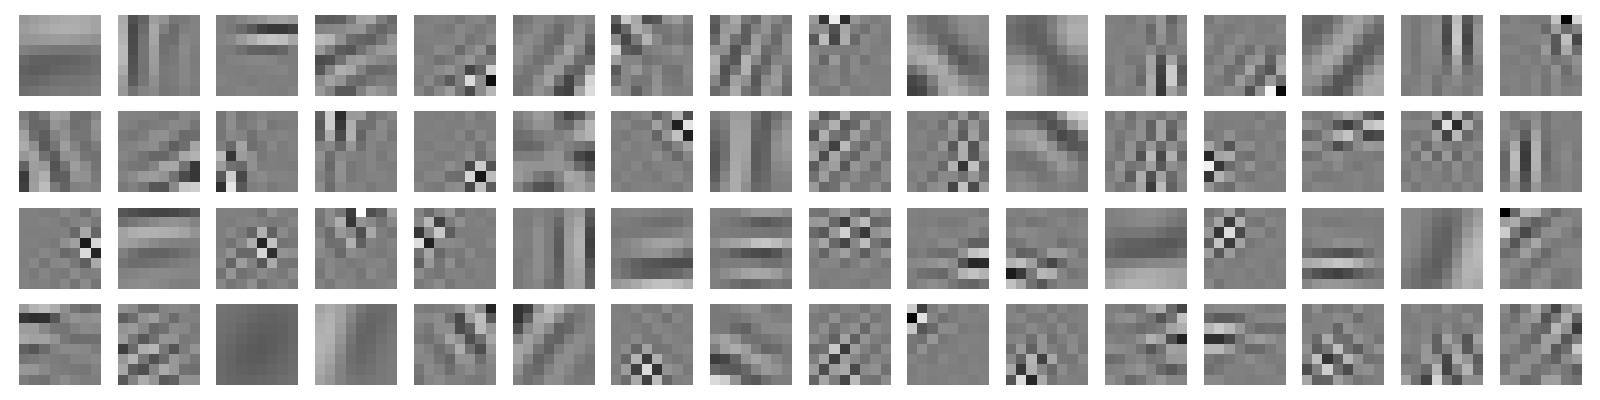
\includegraphics[width=\linewidth]{\toplevelprefix/chapters/chapter2/figs/msp_atoms_patches_new.png}
        \caption{}
    \end{subfigure}
    \begin{subfigure}{0.9\linewidth}
        \centering
        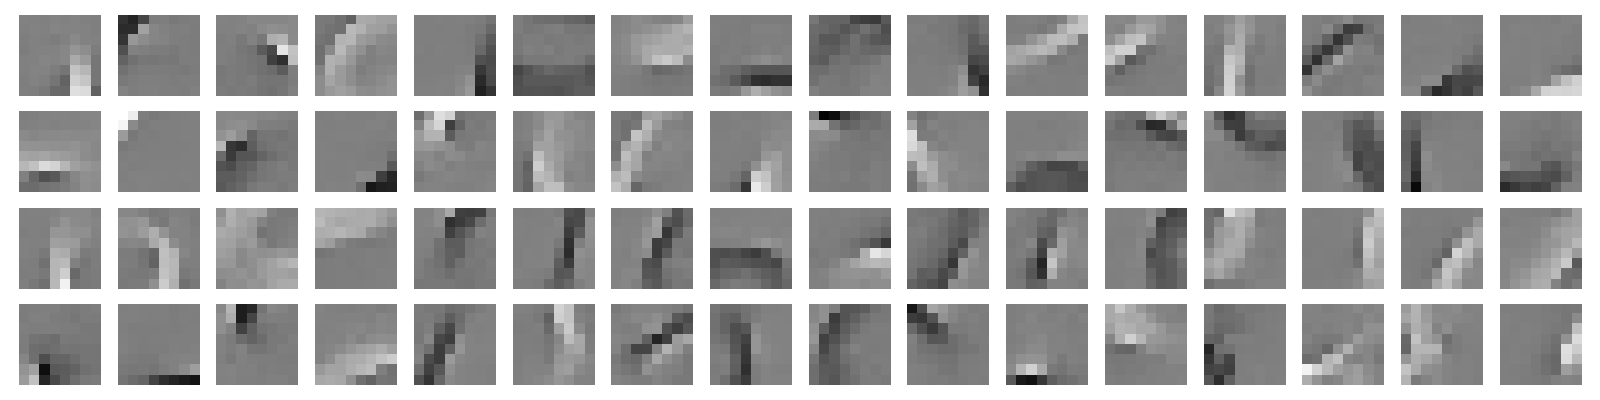
\includegraphics[width=\linewidth]{\toplevelprefix/chapters/chapter2/figs/palm_atoms_patches_new.png}
        \caption{}
    \end{subfigure}
    \caption{Comparison of learned dictionary atoms for complete (orthogonal)
    and overcomplete dictionaries, trained to reconstruct $8$ by $8$ patches taken from
    MNIST digits. Both dictionaries are trained for $6000$ epochs on $10^4$ random patches with
    nontrivial content, and sparse codes are computed with the LASSO objective
    and $\lambda=0.1$ (see \eqref{eq:sparse_dl_lasso}). Colormaps have black for negative values, and white for
    positive values. \textbf{Top:} An orthogonal dictionary learned with the
    MSP algorithm \eqref{eq:msp_iteration} is constrained to
    have no more than $64$ atoms; the learned atoms roughly correspond to
    a ``spike and slab'' dictionary, and achieve relatively poor reconstruction sparsity
    levels on held-out test data (codes are approximately $17$-sparse on
    average, with respect to a threshold of $10^{-1}$).
    \textbf{Bottom:} In contrast, an overcomplete dictionary (here, with $8^3$
    atoms; we visualize a random subset of $64$) learns
    semantically-meaningful dictionary atoms corresponding to signed oriented
    edges, which can be pieced together to create digit patches and achieve
    superior reconstruction and sparisty levels. Codes are approximately
    $20$-sparse on
    average, while being $8$ times larger than those of the orthogonal
    dictionary. To compute the
    dictionary, we use an optimizer based on proximal alternating linearized
    minimization on a suitably-regularized version of
    \eqref{eqn:DL-overcomplete}.}
    \label{fig:ReconMNIST}
\end{figure}

In fact, overcomplete dictionary learning was originally proposed as a biologically plausible algorithm for image representation based on empirical evidence of how early stages of the visual cortex represent visual stimuli \cite{Olshausen1996-ap,Olshausen1997-yv}. 

In the remainder of this section, we will develop the conceptual and computational foundations of overcomplete dictionary learning.
In analogy to the orthogonal dictionary learning problem \eqref{eqn:autoencoding-DL}, we state the compressive autoencoding problem for sparsely-used overcomplete dictionaries. Namely, supposing that the model \eqref{eq:model-DL-overcomplete} is satisfied with data \(\vx\), overcomplete dictionary \(\vA\), and sparsity level \(d\), and given samples \(\vX = [\vx_1, \dots, \vx_N]\) of \(\vx\), we want to learn an encoder \(\cE : \R^D \to \R^m\) mapping each \(\vx\) to its \textit{sparse code} \(\vz\), and a decoder \(\cD(\vz) = \vA \vz\) reconstructing each \(\vx\) from its sparse code, so that \(\cE(\vx)\) and \(\cD(\vz) = \vA\vz\) forms a lossy autoencoding pair for \(\vx\). Pictorially:
\begin{equation}
\x \xrightarrow{\hspace{4mm} \mathcal{E} \hspace{4mm}}  \z \xrightarrow{\hspace{2mm} \mathcal{D} = \vA \hspace{2mm}}   \hat{\x}.  
\label{eqn:autoencoding-DL-overcomplete}
\end{equation}    
We will start from the construction of the encoder $\cE$.
We will work incrementally: first, \textit{given the true dictionary $\vA$}, we will show how the problem of \textit{sparse coding} gives an elegant, scalable, and provably-correct algorithm for recovering the sparse code $\vz$ of $\vx$.
Although this problem is NP-hard in the worst case, it can be solved efficiently and scalably for dictionaries $\vA$ which are \textit{incoherent}, i.e.\ having columns that are not too correlated.
The encoder architecture encompassed by this solution will no longer be symmetric: we will see it has the form of a primitive deep network, which depends on the dictionary $\vA$.
Then we will proceed to the task of learning the decoder $\cD$, or equivalently the overcomplete dictionary $\vA$.
We will derive an algorithm for overcomplete dictionary learning that allows us 
to simultaneously learn the codebook $\vA$ and the sparse codes $\vz$, using ideas from sparse coding.
Finally, we will discuss a more modern perspective on learnable sparse coding that leads us to a fully asymmetric encoder-decoder structure, as an alternative to \eqref{eqn:autoencoding-DL-overcomplete}.
Here, the decoder will correspond to an incremental solution to the sparse dictionary learning problem, and yield for the first time a pair of deep network-like encoder decoders for sparse dictionary learning.
This structure will foreshadow many developments to come in the remainder of the monograph.



%Previously, we had modeled our data, in \(\R^{D}\) as coming from one subspace (Section \ref{sec:lowrank}) or a mixture of up to \(D\) subspaces (Section \ref{sec:ica}). However, this does not yet consider every case where the data has linear structure. Consider the following relevant case. Suppose we have a dataset \(\{\vx_{i}\}_{i = 1}^{N}\) in which the data share certain characteristics; for example, suppose they are all natural images of bedrooms. Then there are a set of common, repeating \textit{motifs} or \textit{patterns} present in nearly all the data: wall painting patterns, beds, dressers, etc. We want to extract those patterns and understand how they combine to form the data. While this seems like a toy example, it occurs all the time in image processing. Famously, the patterns extracted from natural image data using the methods which follow in this chapter are similar to those found in the brain when processing the same data. \DP{cite bruno's paper which applies DL to extract Gabor wavelets from brain data}
%
%More generally, suppose that the data \(\vx_{i}\) all lie in some set \(\cX \subseteq \R^{D}\) (in the above example, the set of natural images of bedrooms). To extract meaning from \(\vx_{i}\) via data analysis, we construct a set of \(d\) \textit{atoms} \(\{\va_{i}\}_{i = 1}^{d} \subseteq \cX\) representing a few interpretable motifs, such that no \(\vx_{i}\) is too far from an atom or a simple (linear) combination of a few atoms such that the motifs combine to form our data. (This is called a \textit{covering}, when formalized, and the number \(d\) is at least the \textit{covering number}, usually much larger than \(D\)). Then, we want to recover an encoding of the \(\vx_{i}\) into the atoms. We also may want to extract an optimal set of atoms, given a dataset. This is the purpose of sparse coding and dictionary learning, respectively.
%%\DP{fill in concrete motivation for sparse coding/dictionary learning later... I think a lot of the examples I give are pretty complicated...}

\subsection{Sparse Coding with an Overcomplete Dictionary} 

In this section, we will consider a data model which accommodates sparse linear combinations of many motifs, or \textit{atoms}. Mechanically, this suggests that we consider the following data model. We say that data \(\{\vx_{i}\}_{i = 1}^{N} \subseteq \R^{D}\) have (approximate) \(s\)-sparse coding structure if and only if there exists a matrix \(\vA = \mat{\va_{1}, \dots, \va_{d}} \in \R^{D \times d}\), vectors \(\{\vz_{i}\}_{i = 1}^{N} \subseteq \R^{d}\) with \(\norm{\vz_{i}}_{0} \leq s\) for all \(i\), and small vectors \(\{\veps_{i}\}_{i = 1}^{N} \subseteq \R^{D}\) such that
\begin{equation}\label{eq:vectorized_sparse_dl_dgp}
    \vx_{i} = \vA\vz_{i} + \veps_{i}, \qquad \forall i \in [N].
\end{equation}
Note the mechanical difference between the sparse coding structure and the principal components structure: 1. the low-dimensional representations \(\vz_{i}\) are required to be \(s\) sparse, and 2. \(\vA\) is not required to be orthogonal. 

The \(s\)-sparsity condition comes from the desire for each data point to be representable by a linear combination of a small number \(s\) of atoms (i.e. columns of \(\vA\)). This essentially imposes that the intrinsic dimension of the data distribution is lower than \(s\).

The relaxing of the orthogonality condition is because, as in our covering example above, \(d\) is much larger than \(D\) and it is impossible to build an orthogonal matrix of size \(D \times d\). Nevertheless, the dictionary \(\vA\), which is either given or learned, is often \textit{incoherent} in the sense that products \(\va_{i}^{\top}\va_{j}\) are often small, hence nearly orthogonal.\footnote{As it turns out, in a high-dimensional space, it is rather easy to pack a number of nearly orthogonal vectors that is much larger than the ambient dimension \cite{Wright-Ma-2022}. } 

Note that we can collect the \(\vx_{i}\) into \(\vX = \mat{\vx_{1}, \dots, \vx_{N}} \in \R^{D \times N}\), collect the \(\vz_{i}\) into \(\vZ = \mat{\vz_{1}, \dots, \vz_{N}} \in \R^{d  \times N}\), and collect the \(\veps_{i}\) into \(\vE = \mat{\veps_{1}, \dots, \veps_{N}} \in \R^{D \times N}\), to rewrite \eqref{eq:vectorized_sparse_dl_dgp} as 
\begin{equation}\label{eq:sparse_dl_dgp}
    \vX = \vA\vZ + \vE.
\end{equation}
The first problem we consider is: what if we know the \(\vA\) matrix, and want to represent our data \(\vX\) using the \(\vA\)? This is the purview of \textit{sparse coding}. Similar to orthogonal dictionary learning, we attempt to find the sparsest signals that are consistent with our observations, and this naturally leads to the following optimization problem:
\begin{equation}\label{eq:sparse_dl_lasso}
    \min_{\vZ \in \R^{d \times N}}\bc{\norm{\vX - \vA\vZ}_{2}^{2} + \lambda \norm{\vZ}_{1}},
\end{equation}
where the \(\ell^1\) norm \(\norm{\vZ}_{1}\) is known to promote sparsity of the solution \cite{Wright-Ma-2022}. 
This problem is known as the LASSO problem. However, unlike the PCA or the
complete dictionary learning case, there is no clear power iteration-type
algorithm to recover \(\vZ^{\star}\). A natural alternative is to consider
solving the above optimization problem with gradient descent type algorithms.
Let \(f(\vZ) = \norm{\vX - \vA\vZ}_{2}^{2} + \lambda \norm{\vZ}_{1}\).
Conceptually we could try to find \(\vZ^{\star}\) with the following iterations:
\begin{equation}
    \vZ_{t+1} \leftarrow \vZ_t + \eta \nabla f(\vZ_t).
\end{equation}

However, because the term associated with the \(\ell^1\) norm \(\norm{\vZ}_{1}\) is non-smooth, we cannot just run gradient descent. For this type of functions, we need to replace the gradient \(\nabla f(\vZ)\) with something that generalizes the notion of gradient, known as the subgradient \(\partial f(\vZ)\):
\begin{equation}
    \vZ_{t+1} \leftarrow \vZ_t + \eta \partial f(\vZ_t).
\end{equation}
However, it is known that the convergence of subgradient descent is usually very slow. Hence, for this type of optimization problems, it is conventional to adopt a so-called {\em proximal gradient descent}-type algorithm. One may refer to \cite{Wright-Ma-2022} for a detailed introduction to this method. 

Applying proximal gradient to the LASSO objective function \eqref{eq:sparse_dl_lasso}, it leads to the classic \textit{iterative shrinkage-thresholding algorithm} (ISTA), which implements the iteration
\begin{eqnarray}
    \vZ_{1} &\sim& \dNorm(\vzero, \vI), \\
    \vZ_{t + 1} &=& S_{\eta\lambda}\rp{\vZ_{t} - 2\eta \vA^{\top}(\vA\vZ_{t} - \vX)}, \quad \forall t \geq 1,\label{eq:ista_update}
\end{eqnarray}
with step size \(\eta \geq 0\), and the soft-thresholding operator \(S_{\alpha}\) defined on scalars by
\begin{equation}
    S_{\alpha}(x) \doteq \begin{cases}x - \alpha, & x \geq \alpha, \\ 0, & -\alpha < x < \alpha, \\ x + \alpha, & x \leq -\alpha\end{cases},
\end{equation}
and applied element-wise to the input matrix.  As a proximal gradient descent algorithm applied to a convex problem, convergence to a global optimum is assured, and convergence rate can be derived straightforwardly \cite{Wright-Ma-2022}. 

We now take a moment to remark on the functional form of the update operator in \eqref{eq:ista_update}, it takes the form 
\begin{equation}
    \vZ_{t + 1} = \texttt{nonlinearity}(\vZ_{t} + \texttt{linear}^{\top}(\texttt{linear}(\vZ_{t}) + \texttt{bias})).
\end{equation}
This functional form is very similar to that of a residual network layer, namely,
\begin{equation}
    \vZ_{t + 1} = \vZ_{t} + \texttt{linear}_{1}^{\top}(\texttt{nonlinearity}(\texttt{linear}_{2}(\vZ_{t}) + \texttt{bias}_{1}) + \texttt{bias}_{2},
\end{equation}
only decoupling the linear maps (i.e., matrix multiplications), adding a bias, and moving the nonlinearity. The ISTA, then, can be viewed as a forward pass of a primitive (recurrent one-layer) neural network. We argue in Chapter \ref{ch:representation} that such operations are essential to deep representation learning.

% Mixture of low-dim linear independent structures.... Lasso and L1 minimization. Introduce basic algorithm for sparse coding such as ISTA.

% \begin{itemize}
%     \item Motivate LASSO/L1 as: first we understand ICA as multiple subspaces where we only sum from a few subspace basis vectors at a time. Now what if we just send number of subspace basis vectors to \(\infty\)? Or very large? Becomes sparse representation problem
%     \item Introduce LASSO and ISTA
%     \item When we do have the dictionary it's LASSO and L1, when we don't, it's overcomplete dictionary learning, discuss LISTA/KSVD etc and applications
% \end{itemize}


\subsection{Overcomplete Dictionary Learning} 

Recall that we have the data model 
\begin{equation}
    \vX = \vA\vZ + \vE,
\end{equation}
where \(\vZ\) is sparse, and our goal previously was to estimate \(\vZ\) given knowledge of the data \(\vX\) and the dictionary atoms \(\vA\). Now we turn to the more usual, more natural, and more difficult case where we do not know either \(\vA\) or \(\vZ\) and seek to learn them from a large dataset. In particular, we solve the problem
\begin{equation}
    \min_{\tilde{\vA}, \tilde{\vZ}}\bc{\norm{\vX - \tilde{\vA}\tilde{\vZ}}_{F}^{2} + \lambda \norm{\tilde{\vZ}}_{1}}.
    \label{eqn:DL-overcomplete}
\end{equation}
\begin{remark}[$\ell^4$ maximation versus $\ell^1$ minimization]
Note that the above problem formulation follows naturally from the LASSO formulation \eqref{eq:sparse_dl_lasso} for sparse coding. We promote the sparsity of the solution with minimizing the \(\ell^1\) norm. Nevertheless, if we are only interested in recovering the over-complete dictionary \(\vA\), the \(\ell^4\) maximization scheme introduced in Section \ref{sec:complete-dictionary} also generalizes to the over-complete case, without any significant modification. Interested readers may refer to the work of \cite{Qu2020Geometric}. 
\end{remark}

The above problem \eqref{eqn:DL-overcomplete}, which we call \textit{overcomplete dictionary learning}, is nonconvex as here both \(\vA\) and \(\vZ\) are unknown now. We cannot be solved easily by the standard convex optimization toolkit. Nevertheless, because it is interesting, simple to state, and practically important, there have been many important works dedicated to different algorithms and theoretical analysis for this problem. Here, for the interest of this book, we present an idiomatic approach to solve this problem which is closer to the spirit of deep learning.

From our experience with the LASSO problem above, it is easy to see that, for the two unknowns \(\vA\) and \(\vZ\), if we fix one and optimize the other, each subproblem is in fact convex and easy to solve. This naturally suggests that we could attempt to solve the above program \eqref{eqn:DL-overcomplete} by minimizing against \(\vZ\) or \(\vA\) alternatively, say using gradient descent. This leads to the following iterative scheme:
\begin{align}
    & \vZ^{1}
     \sim \dNorm(\vzero, \vI), \quad \vA_{1}
     \sim \dNorm(\vzero, \vI), \\ 
    &\vZ^{\ell + 1} = S_{\eta\lambda}\rp{\vZ^{\ell} - 2\eta\vA_{t}^{\top}(\vA_{t}\vZ^{\ell} - \vX)}, \qquad \forall \ell \in [L] \label{eqn:ISTA-update}\\ 
    &\vA_{t + 1} = \vA_{t} - 2\nu (\vA_{t}\vZ^{\ell + 1} - \vX)\vZ^{\ell + 1}, \qquad\;\; \forall t \in [T].\label{eqn:DL-update}
\end{align}
Here, unlike typically alternating minimization scheme, we here use two separate indices $\{t\}$ and $\{\ell\}$ to indicate the iterations. As we will see later, this allows us to interpret the two updates separately in the context of deep learning. Despite the dictionary learning problem is a nonconvex problem, it has been shown that the above alternating minimization type algorithms indeed converge to the correct solution, at least locally, see for example \cite{alekh-2016}.

%\yima{Sam, please fix this as a vanilla algorithm for solving the over-complete dictionary learning problem. State results regarding understanding the correctness of such an approach... Complete this subsection.}

\subsection{Learned Deep Sparse Coding}
\label{sec:LISTA}
The main observation from the above approach is to notice that \textit{when we fix \(\vA\), the ISTA update for $\vZ^\ell$ \eqref{eqn:ISTA-update} looks like the forward pass of a deep neural network with weights given by \(\vA\) (and \(\vA^{\top}\))}. But in general, we do not know the true $\vA_o$, and the current estimate $\vA_t$ could be erroneous. Hence it needs to be further updated using \eqref{eqn:DL-update} based on the residual of using the current $\vA_t$ and $\vZ^{\ell +1}$ to recover $\vX$. 


\paragraph{Layerwise learned sparse coding.}
Hence, if we view each ISTA update \eqref{eqn:ISTA-update} as a layer and allow the associated dictionary, now denoted as $\vA_t^\ell$, to update in time, this leads to a  ``layerwise-learnable'' sparse coding scheme:
\begin{align}
    & \vZ^{\ell + 1} = S_{\eta\lambda}\rp{\vZ^{\ell} - 2\eta\vA_{t}^{\ell\top}(\vA_{t}^\ell\vZ^{\ell} - \vX)}, \quad \forall \ell \in [L] \\ 
    & \vA_{t + 1}^\ell = \vA_{t}^\ell - 2\nu (\vA_{t}^\ell\vZ^{\ell + 1} - \vX)\vZ^{\ell + 1}, \qquad \forall t \in [T].
\end{align}
Each of the \(L\) inner steps can be considered as a one-layer  forward pass, while each of  the \(T\) outer steps can be considered as a one-layer  backward pass, of a primitive deep neural network. In particular, this algorithm is the simplest case in which a clear divide between forward optimization and backward learning manifests. This divide is still observed in current neural networks.

\paragraph{Learned ISTA.} The above deep-network  interpretation of the alternating minimization is more conceptual than practical, as the process could be rather inefficient and take many layers or iterations to converge. But this is mainly because we try to infer both \(\vZ\) and \(\vA\) from \(\vX\). The problem can be significantly simplified and the above iterations can be made much more efficient if we only use them to learn \(\vA^\ell\) from a given set of samples of input and output  \((\vX, \vZ)\) for the iterative sparse encoding:
\begin{align}
    & \vZ^{\ell + 1} = S_{\eta\lambda}\rp{\vZ^{\ell} - 2\eta(\vA^{\ell})^{\top}(\vA^\ell\vZ^{\ell} - \vX)}, \quad \forall \ell \in [L].
\end{align}
If we denote the operator for each iteration as $\vZ^{\ell + 1} = f(\vA^\ell, \vZ^\ell)$, the above iteration can be illustrated in terms of a diagram:
\begin{equation*}
\vX, \vZ^1 \xrightarrow{\hspace{1mm} f(\vA^1,\,\cdot\,) \hspace{1mm}}  \vZ^2 \xrightarrow{\hspace{1mm} f(\vA^2,\,\cdot\,) \hspace{1mm}}  \vZ^3  \xrightarrow{\hspace{1mm} f(\vA^3,\,\cdot\,) \hspace{1mm}} \cdots \vZ^{L}  \xrightarrow{\hspace{1mm} f(\vA^{L},\,\cdot\,) \hspace{1mm}} \vZ^{L + 1} \approx \vZ.  
\label{eqn:deep-sparse-encoding}
\end{equation*}

Thus, given the sequential architecture, to learn the operator \(\vA^\ell\) at each layer, it is completely natural to learn it, say via back propagation (BP),\footnote{See Appendix \ref{app:optimization} for a brief description of BP.} by minimizing the error between the final code $\vZ^L$ and the ground truth $\vZ$:
\begin{equation}
    \min_{\{\vA^\ell\}} \big\|\vZ^L(\vA^1, \ldots, \vA^{L}) - \vZ\big\|_2^2.
\end{equation}
This is the basis of the Learned ISTA (LISTA) algorithm \cite{gregor2010learning}, which can be viewed as the learning algorithm for a deep  neural network, which tries to emulate the sparse encoding process from $\vX$ to $\vZ$. In particular, it can be viewed as a \textit{simple representation learning algorithm}. 
%\yima{probably spell out LISTA as an algorithm in pseudo code form.}


The empirical success of LISTA begs the question: what if we use layer-wise different  dictionaries \(\vA^\ell\) to encode even more complicated data, and learn the weights via backpropagation? This is \textit{exactly} the idea behind deep (linear) neural networks. We will discuss this more in subsequent Chapters.

% Mixture of low-dim linear independent structures without knowing the encoding,... L4 maximization. Our work on the complete case: \href{https://arxiv.org/abs/1906.02435}{L4-based dictionary learning} 





\section{Summary and Notes}


\sdb{Add some short summary and a table that summarizes the power methods. Maybe this section should go at the end of the chapter instead, along with the autoencoding summary table?}

\textit{Independent component analysis} (ICA), was proposed by \cite{Ans-1985} and pioneered by Aapo Hyv\"{a}rinen in the 1990s and early 2000s.

Unified computational mechanisms: Pursuit of low-dimensional linear and independent models via {\em power iteration} based on first-order oracles (gradients). 

Mention early history of using autoassociative or autoencoding neural networks to learn PCA and probably recent work by Qing's group on learn PCA via diffusion. 

Mention the work from John Wright and Qing Qu etc. on the over-complete dictionary learning.

Mention early generalizations to multiple subspaces (e.g. GPCA) and their limitations, and connections to later chapters on Rate Reduction.


\section{Exercises and Extensions}


\begin{exercise}\label{exercise:principal-components-derivation}
    Prove that, for any symmetric matrix \(\vA\), the solution to the problem
    \(\max_{\vU \in \O(D, d)}\tr\left(\vU^{\top}\vA\vU\right)\) is the matrix
    \(\vU^{\star}\) whose columns are the top \(d\) unit eigenvectors of \(\vA\).
\end{exercise}

\begin{exercise}\label{exercise:gaussian-rot-invar}
    Let $\vz \sim \cN(\Zero, \sigma^2 \vI)$ be a Gaussian random variable with independent components, each with variance $\sigma^2$. 
    Prove that for any orthogonal matrix $\vQ$ (i.e., $\vQ^\top \vQ = \vI$), the random variable $\vQ \vz$ is distributed identically to $\vz$. 
    \textit{(Hint: recall the formula for the Gaussian probability density function, and the formula for the density of a linear function of a random variable.) }
\end{exercise}

\begin{exercise}\label{exercise:symmetry-identifiability}
    The notion of statistical identifiability discussed above can be related to \textit{symmetries} of the model class, allowing estimation to be understood in a purely deterministic fashion without any statistical assumptions.

    Consider the model $\vX = \vU \vZ$ for matrices $\vX, \vU, \vZ$ of compatible sizes.
    \begin{enumerate}
        \item Show that if $\vA$ is any square invertible matrix of compatible size, then the pair
        $(\vU \vA, \vA^{-1} \vZ)$ also equals $\vX$ under the model. We call this a \textit{$\GL(d)$ symmetry}.
        \item Suppose each column of $\vZ$ is an independent and identically distributed observation from a common statistical model $\vz$, which moreover has zero mean and independent components $z_i$ with positive variance.
        Show that for any square invertible matrix $\vA$, if $\vA \vz$ has uncorrelated components, then $\vA$ can be written as $\vD_1 \vQ \vD_2$, where $\vQ$ is an orthogonal matrix and $\vD_1$, $\vD_2$ are diagonal matrices.
        \textit{This links the ``independence'' assumption in ICA to a ``symmetry breaking'' effect, which only allows scale and rotational symmetries.}
    \end{enumerate}

\end{exercise}

\begin{exercise}\label{exercise:whitening}
    Consider the model $\vx = \vU \vz$, where $\vU \in \R^{D \times d}$ with $D \geq d$ is fixed and has rank $d$, and $\vz$ is a zero-mean random variable. Let $\vx_1, \dots \vx_N$ denote i.i.d.\ observations from this model.
    \begin{enumerate}
        \item Show that the matrix $\vX = [\vx_1, \dots, \vx_N]$ has rank no larger than $d$, and therefore there is an orthonormal matrix $\vV \in \R^{D \times d}$ so that $\vX = \vV \vY$, where $\vY \in \R^{d \times N}$. (\textit{Hint: use PCA.})
        \item Show that the \textit{whitened matrix} $(\vY \vY^\top)^{-1/2}\vY$ exists in expectation whenever $\Cov(\vz)$ is nonsingular, and that it has identity empirical covariance.\footnote{In particular, it can be proved mathematically that this is enough to guarantee that the whitened matrix exists with high probability whenever $\vz$ satisfies a suitable concentration inequality and $N$ is sufficiently large.}
        \item Show, by using the singular value decomposition of $\vU$, that the matrix $\vV$ can be chosen so that the whitened matrix satisfies $(\vY \vY^\top)^{-1/2} \vY = \vW [\vz_1, \dots, \vz_N]$, where $\vW$ is an orthonormal matrix.
    \end{enumerate}
\end{exercise}

\begin{exercise}\label{exercise:kurtosis-linearity-properties}
    Let $X$ and $Y$ be zero-mean independent random variables.
    \begin{enumerate}
        \item Show that $\kurt(X + Y) = \kurt(X) + \kurt(Y)$.
        \item For any $\alpha \in \R$, show that $\kurt(\alpha X) = \alpha^4 \kurt(X)$.
    \end{enumerate}
\end{exercise}

\begin{exercise}\label{exercise:sphere-calculus}
    Let $f : \R^d \to \R$ be a given twice-continuously-differentiable objective function. Consider the spherically-constrained optimization problem
    \begin{equation}\label{eq:exercise-sphere-constrained-max}
        \max_{\norm{\vu}_2^2 = 1}\, f(\vu). 
    \end{equation}
    In this exercise, we will derive the expressions we gave in the FastICA derivation for maximizing kurtosis over the sphere via a gradient ascent algorithm.
    These expressions are special cases of a rich theory of calculus and optimization on manifolds, of which the sphere is a particular example. A deep technical study of this field is out-of-scope for our purposes, so we only mention two key references for the interested reader: the pioneering textbook by Absil, Mahony, and Sepulchre
    \cite{Absil2009-nc}, and a more recent introductory treatise by Boumal \cite{Boumal2023-rj}. 
    \begin{enumerate}
        \item For any constraint set $\cM$ that is a differentiable submanifold of $\R^d$, the 
        \textit{tangent space} at a point $\vu \in \cM$ is, informally, the best local linear approximation to the manifold $\cM$ at the point $\vu$.
        In the important special case where $\cM$ is defined locally at $\vu$ as a level set of a function $F : \R^d \to \R$,
        that is
        \begin{equation*}
            U \cap \cM = F^{-1}(\set{0})
        \end{equation*}
        for some open set $U \subset \cM$ with $\vu \in U$,
        the tangent space to $\cM$ at $\vu$ can be calculated 
        via differentiation:
        \begin{equation*}
            T_{\vu} \cM = \Ker(DF_{\vu}).
        \end{equation*}
        It is easily seen that the sphere has the defining equation $F(\vu) = \norm{\vu}_2^2 - 1$.
        Show, using these facts, that the tangent space to the sphere at $\vu$ is given by
        \begin{equation*}
            T_{\vu} \bS^{d-1} = \set{\vv \in \R^d \given \ip{\vv}{\vu} = 0},
        \end{equation*}
        and that the orthogonal projection onto this subspace is $\vP_{\vu}^\perp = \vI - \vu\vu^\top$.
        \item The vector field 
        \begin{equation}\label{eq:exercise-riemann-grad-sphere}
        \mathrm{grad}\, f(\vu) = \vP_{\vu}^\perp \nabla f
        \end{equation}
        is known as the \textit{Riemannian gradient} of the function $f$ restricted to the sphere.
        The \textit{first order optimality conditions} for the optimization problem \eqref{eq:exercise-sphere-constrained-max} can be expressed in terms of the Riemann gradient:
        \begin{equation*}
            \mathrm{grad}\, f(\vu) = \mathbf{0}.
        \end{equation*}
        Geometrically, this says that the Euclidean gradient of $f$ at $\vu$ must be orthogonal to the tangent space to the sphere at $\vu$.
        Now suppose $\vv \in \R^d$ is nonzero. Show that
        \begin{equation*}
            \mathrm{proj}_{\bS^{d-1}}(\vv) :=
            \min_{\norm{\vu}_2^2 = 1}\, \norm{\vu - \vv}_2 
            =
            \frac{\vv}{\norm{\vv}_2},
        \end{equation*}
        using the first-order optimality conditions. 
        \item In optimization over $\R^d$, one checks the second-order optimality conditions (to determine whether a critical point is a maximizer, a minimizer, or a saddle point) using the \textit{Hessian matrix} $\nabla^2 f(\vu)$.
        Show, by differentiating the Riemann gradient $\mathrm{grad}\, f(\vu)$ for the sphere with respect to $\vu$ as in the first part of this exercise, that the corresponding object for determining second-order optimality conditions for sphere-constrained optimization is the \textit{Riemannian Hessian}, defined as
        \begin{equation}\label{eq:exercise-riemann-hess-sphere}
            \mathrm{Hess}\, f(\vu) = \vP_{\vu}^\perp \left( 
            \nabla^2 f(\vu) - \ip{\nabla f(\vu)}{\vu} \vI
            \right) \vP_{\vu}^\perp.
        \end{equation}
    \end{enumerate}
\end{exercise}

\begin{exercise}\label{exercise:kurtosis-sphere-landscape}
    In this exercise, we sketch an argument referred to in the literature as a \textit{landscape analysis} for the spherically-constrained population kurtosis maximization problem \eqref{eq:kurtosis-maximization-sphere-population-simple}. We will show that when there is at least one independent component with positive kurtosis, its 
    global maximizers indeed lead to the recovery of one column of the dictionary $\vU$.
    For simplicity, we will assume that $\kurt(z_i) \neq 0$ for each $i = 1, \dots, d$.
    \begin{enumerate}
        %\item Using the running assumption $\Var(z_i) = 1$, show that $\kurt(z_i) = \bE[z_i^4] - 3$.
        \item Using the results of Part 1 of Exercise \ref{exercise:sphere-calculus}, 
        show that the first-order optimality condition for \eqref{eq:kurtosis-maximization-sphere-population-simple} is
        \begin{equation}\label{eq:kurtosis-sphere-landscape-stationarity}
            \left(\sum_{i=1}^d \kurt(z_i) w_i^4 \right) 
            \vw = \kurt(\vz) \hada \vw^{\hada 3}, 
        \end{equation}
        where the kurtosis is calculated elementwise, $\hada$ denotes elementwise multiplication of vectors and $\vw^{\hada 3}$ denotes the elementwise cube of its argument.
        \item Show that the vectors $\vw$ with unit norm that also satisfy \eqref{eq:kurtosis-sphere-landscape-stationarity}
        all take the following form.
        Let $S^+ = \set{i \in [d] \given \kurt(z_i) > 0}$, and 
        $S^- = \set{i \in [d] \given \kurt(z_i) < 0}$.
        Let $S$ be a subset either of $S^+$ or $S^-$.
        Then 
        \begin{equation}\label{eq:kurtosis-sphere-landscape-cps}
            \vw_S = \sum_{i \in S} \pm \sqrt{\frac{1}{\kurt(z_i) \sum_{j \in S} \frac{1}{\kurt(z_j)}}} \ve_i
        \end{equation}
        satisfies \eqref{eq:kurtosis-sphere-landscape-stationarity},
        where $\ve_i$ is the vector with a $1$ in the $i$-th position and $0$s elsewhere, and the $\pm$ sign denotes the choice of either a positive or negative sign.
        \item Assume that there is at least one $i$ such that $\kurt(z_i) > 0$. Using the results of Part 2 of Exercise \ref{exercise:sphere-calculus}, show that the only local maxima of the objective of \eqref{eq:kurtosis-maximization-sphere-population-simple} are the signed one-sparse vectors $\pm \ve_i$ with $i \in S^+$. Conclude that the global maximizers of \eqref{eq:kurtosis-maximization-sphere-population-simple} are the signed one-sparse vectors corresponding to components with maximum kurtosis. %
        %Let $S_{\max} = \argmax_{i \in [d]}\, \kurt(z_i)$ be the set of indices of independent components with maximum kurtosis. Then for each $i \in S_{\max}$, $\pm \ve_i$ is a local maximizer of \eqref{eq:kurtosis-maximization-sphere-population-simple}.
        (\textit{Hint: count the number of positive and negative eigenvalues of the Riemannian Hessian \eqref{eq:exercise-riemann-hess-sphere} at each critical point.})
        %\item Show that the value of the objective of \eqref{eq:kurtosis-maximization-sphere-population-simple} at any critical point $\vw_S$ defined above is given by
        %\begin{equation*}
        %    \frac{1}{\sum_{i \in S} \frac{1}{\kurt(z_i)}}.
        %\end{equation*}
        %\item Conclude that the 
        \item Now assume that $\kurt(z_j) < 0$ for every $j =1, \dots, d$. This corresponds to an ``over-deflated'' instantiation of the kurtosis maximization problem. Using again the results of Part 2 of Exercise \ref{exercise:sphere-calculus}, show that the only local maxima of the objective of \eqref{eq:kurtosis-maximization-sphere-population-simple} are the signed dense vectors $\sum_{i=1}^d \pm \ve_i$.
        This shows that the optimization formulation \eqref{eq:kurtosis-maximization-sphere-population-simple} cannot be applied naively.
    \end{enumerate}
\end{exercise}

\begin{exercise}\label{exercise:fast-ica-convergence}
    \sdb{Convergence of fastica, based on \cite{hyvarinen-1997}, section 3.2} 
\end{exercise}

%\begin{exercise}\label{exercise:orthogonal-dl-simplifying}
%    \sdb{simplify the orthogonal DL LASSO loss... rotation invariance of $\ell^2$, then separability, then Huber calculation}
%\end{exercise}

\begin{exercise}\label{exercise:orthogonal-group-calculus}
    This exercise follows the structure and formalism introduced in Exercise \ref{exercise:sphere-calculus}, but applies it instead to the orthogonal group $\O(d) = \set{\vU \in \R^{d \times d} \given \vU^\top \vU = \vI}$. 
    Consult the description of Exercise \ref{exercise:sphere-calculus} for the necessary conceptual background; the formalism applies identically to the case where the ambient space is the set of $d \times d$ matrices as long as one recalls that the relevant inner product on matrices is $\ip{\vX}{\vY} = \tr(\vX^\top \vY)$.
    An excellent general reference for facts about optimization on the orthogonal group is Edelman, Arias, and Smith \cite{Edelman1998-lg}.
    
    Let $f : \R^{d\times d} \to \R$ be a given twice-continuously-differentiable objective function. Consider the orthogonally-constrained optimization problem
    \begin{equation}\label{eq:exercise-orthogonal-group-constrained-max}
        \max_{\vQ^\top \vQ = \vI}\, f(\vQ). 
    \end{equation}
    \begin{enumerate}
        \item  It is easily seen that the orthogonal group has the defining equation $F(\vQ) = \vQ^\top \vQ = \vI$.
        Show, using this fact, that the tangent space to the orthogonal group at $\vQ$ is given by
        \begin{equation*}
            T_{\vQ} \O(d) = \set{\vQ \vOmega \in \R^{d\times d} \given \vOmega^\top = - \vOmega},
        \end{equation*}
        and that the orthogonal projection onto this subspace is 
        \begin{equation*}
        \cP_{T_{\vQ}\O(d)}(\vDelta) =  \vQ \Skew(\vQ^\top \vDelta),
        \end{equation*}
        where $\Skew(\vDelta) = \tfrac{1}{2} ( \vDelta - \vDelta^\top)$ is the orthogonal projection onto the set of skew-symmetric matrices.
        The vector field 
        \begin{equation}\label{eq:exercise-riemann-grad-orthogonal-group}
        \mathrm{grad}\, f(\vQ) = \cP_{T_{\vQ} \O(d)} \left( \nabla f(\vQ) \right)
        \end{equation}
        is known as the \textit{Riemannian gradient} of the function $f$ restricted to the orthogonal group.
        The \textit{first order optimality conditions} for the optimization problem \eqref{eq:exercise-orthogonal-group-constrained-max} can be expressed in terms of the Riemann gradient:
        \begin{equation*}
            \mathrm{grad}\, f(\vQ) = \mathbf{0}.
        \end{equation*}
        \item Show, by differentiating the Riemann gradient $\mathrm{grad}\, f(\vQ)$ for the orthogonal group with respect to $\vQ$ as in the first part of this exercise, that the \textit{Riemannian Hessian} is given by
        \begin{equation}\label{eq:exercise-riemann-hess-orthogonal-group}
            \mathrm{Hess}\, f(\vQ) = \cP_{T_{\vQ}\O(d)} \left( 
            \nabla^2 f(\vQ) - \Symm(\vQ^\top \nabla f(\vQ)) \kron \vI
            \right) \cP_{T_{\vQ}\O(d)},
        \end{equation}
        where $\Symm(\vDelta) = \tfrac{1}{2}(\vDelta + \vDelta^\top)$ denotes the orthogonal projection onto the set of symmetric matrices, and $\kron$ denotes the Kronecker product of matrices.
        Take care to interpret the operators appearing in the previous expression as \textit{linear transformations on ${d \times d}$ matrices}, \textbf{not} as $d \times d$ matrices themselves.
        The \textit{second-order optimality conditions} for the optimization problem \eqref{eq:exercise-orthogonal-group-constrained-max} can be expressed in terms of the Riemann Hessian:
        \begin{equation*}
            \mathrm{Hess}\, f(\vQ) \preceq \mathbf{0}.
        \end{equation*}
        For a minimization problem, the sign is reversed.

        (\textit{Hint: The key is to manipulate one's calcluations to obtain the form \eqref{eq:exercise-riemann-hess-orthogonal-group}, which is as compact as possible. To this end, make use of the following isomorphism of the Kronecker product: if $\vA$, $\vX$, and $\vB$ are matrices of compatible sizes, then one has
        \begin{equation*}
            (\vB^\top \kron \vA) \Vec(\vX) = \Vec(\vA \vX \vB),
        \end{equation*}
        where $\Vec(\vX)$ denotes the ``left-to-right'' stacking of the columns of the matrix argument into a vector. We use this isomorphism in \eqref{eq:exercise-riemann-hess-orthogonal-group} in order to define the Kronecker product of two matrices as an operator on matrices in a canonical way.})
        
        \item Now suppose $\vX \in \R^{d\times d}$ is full-rank. In this and the next part of the exercise, we consider the projection onto the orthogonal group of $\vX$:
        \begin{equation}\label{eq:projection-onto-ogrp-defn}
            \mathrm{proj}_{\O(d)}(\vX) :=
            \min_{\vQ \in \O(d)
            }\, \norm{\vQ - \vX}_F^2.
        \end{equation}
        We will prove that the solution to this problem is given by
        \begin{equation*}
            \mathrm{proj}_{\O(d)}(\vX)
            =
            \vU \vV^\top,
        \end{equation*}
        where $\vX = \vU \vS \vV^\top$ is a singular value decomposition of $\vX$. 

        \begin{enumerate}
            \item Using the first and second-order optimality conditions, show that every local minimizer $\vQ$ of \eqref{eq:projection-onto-ogrp-defn} satisfies
            \begin{align*}
                \left( \vQ^\top \vX \right)^\top &= \vQ^\top \vX, \\
                \vQ^\top \vX &\succeq \mathbf{0}.
            \end{align*}
            (\textit{Hint: use linearity of the Kronecker product in either of its two arguments when the other is fixed.})
            \item Using these conditions, argue that at every local minimizer $\vQ$ of \eqref{eq:projection-onto-ogrp-defn}, one has $\vQ^\top \vX = (\vX^\top \vX)^{1/2}$.
            %the loss value achieved is $\norm{(\vX\adj \vX)^{1/2} - \vI}_F^2$.
            (\textit{Hint: Use %unitary invariance of the $\ell^2$ norm and 
            the fact from linear algebra that if $\vS \succeq \mathbf{0}$ is a symmetric positive semidefinite matrix, then $(\vS^\top\vS)^{1/2} = \vS$.})
            \item Using the singular value decomposition $\vX = \vU \vS \vV^\top$, conclude that
            \begin{equation*}
                \vU \vV^\top
                =
                \mathrm{proj}_{\O(d)}(\vX).
            \end{equation*}
        \end{enumerate}
    \end{enumerate}
\end{exercise}

% \begin{exercise}\label{exercise:l4-global-maximizers-ogrp}
% %\sdb{Exercise to derive global maximizers of $\ell^4$ objective. Follow Simon's paper / elementary argument.}
% \end{exercise}

%\begin{exercise}\label{exercise:l4-maximizers-ogrp}
%    As we have seen, the first-order optimality conditions for $\ell^4$ maximization over the orthogonal group (Equation \eqref{eq:l4-ogrp-fxp-step1}) can be written as follows: a point $\vQ$ is a critical point for the objective if and only if
%    \begin{equation}\label{eq:l4-ogrp-fxp-exercise-1}
%        \vX \left( \vX \adj \vQ \right)^{\hada 3} = \vQ \underbrace{\left. \left(
%        \vQ\adj \vX \left( \vX \adj \vQ \right)^{\hada 3} 
%        + 
%        \left( \vQ\adj \vX \right)^{\hada 3} \vX\adj \vQ
%        \right) \right/ 2}_{\vS}.
%    \end{equation}
%    We will show in this exercise that the symmetric matrix $\vS$ defined by this condition is positive semidefinite at any maximizer of the objective.
%    Below, we write $f(\vQ) = \norm{\vX\adj \vQ}_4^4$ for concision.
%    \begin{enumerate}
%        \item Using the expression \eqref{eq:exercise-riemann-hess-orthogonal-group} for the Riemannian Hessian over the orthogonal group derived in Exercise \ref{exercise:orthogonal-group-calculus}, argue that a necessary condition for a point $\vQ$ to be a local maximizer of the $\ell^4$ maximization problem is that $\vQ$ satisfies \eqref{eq:l4-ogrp-fxp-exercise-1} and
%        \begin{equation*}
%            \cP_{T_{\vQ}\O(d)}
%            \left(
%             \vQ\adj \nabla f(\vQ) \kron \vI
%             \right)
%            \cP_{T_{\vQ}\O(d)}
%            \succeq \mathbf{0}.
%        \end{equation*}
%        \item Using the definition of the Kronecker product, argue that the previous condition is equivalent to the following condition: for any skew-symmetric matrix $\vOmega$ (i.e., such that $\vOmega\adj = -\vOmega$), one has
%        \begin{equation*}
%            \ip*{\vOmega}{
%             \vOmega \vQ\adj \nabla f(\vQ)
%             }
%            \geq 0.
%        \end{equation*}
%        (\textit{Hint: recall the definition of the tangent space to the orthogonal group from Exercise \ref{exercise:orthogonal-group-calculus}.})
%        \item By the spectral theorem from linear algebra, any skew-symmetric matrix $\vOmega$ (being a normal matrix) has an eigenvalue decomposition $\vOmega = \vV \vLambda \vV\adj$, where $\vV \in \C^{d \times d}$ is a unitary matrix, and $\vLambda \in \C^{d\times d}$ is a diagonal matrix of eigenvalues. 
%        Prove the following characterization of real-valued skew-symmetric matrices $\vOmega \in \R^{d \times d}$: one has $\vOmega\adj = -\vOmega$ if and only if $\vOmega = \vV \vLambda \vV\adj$ for a unitary matrix $\vV$ and a diagonal matrix $\vLambda$ having the following symmetries:
%        \begin{itemize}
%            \item All eigenvalues $\lambda_i$ are purely imaginary, so that $\mathfrak{R}(\lambda_i) = 0$.
%            \item When $d$ is even, the eigenvalues $\lambda_i$ can be partitioned into pairs with the following property. If $(i, j)$ is a pair of indices in the partition, one has $\lambda_i = -\lambda_j$. When $d$ is odd, the same partition can be formed, but with an additional odd number of indices $i$ such that $\lambda_i = 0$.
%            \item The corresponding eigenvectors $\vv_i$ and $\vv_j$ associated to the nonzero eigenvalues in each pair of this partition satisfy $\vv_i = \ol{\vv_j}$, where $\ol{z}$ denotes the conjugate of a complex number $z$ (applied elementwise to a complex vector).
%            The eigenvectors associated to zero eigenvalues are arbitrary, such that the matrix $\vV$ is unitary.
%        \end{itemize}
%        \item Using the preceding characterization of skew-symmetric matrices and the previous condition for local maxima of the $\ell^4$ maximization problem, 
%        conclude that at any local maximum $\vQ$, one must have
%        \begin{equation*}
%            \vQ\adj \nabla f(\vQ) \succeq \mathbf{0}. 
%        \end{equation*}
%        (\textit{Hint: if $\vOmega$ is skew-symmetric, then by the characterization from the previous part, the semidefinite matrix $\vOmega\adj \vOmega$ has eigenvalues that can be partitioned into pairs of equal value. If $\vv$ is the eigenvector associated to this (nonzero) pair, show that $\mathfrak{R}(\vv)$ and $\mathfrak{I}(\vv)$ (suitably normalized) can be chosen as the corresponding eigenvectors of $\vOmega\adj \vOmega$. Given a putative local maximum $\vQ$ such that $\vQ\adj \nabla f(\vQ) \not \succeq \mathbf{0}$, use this construction to derive a contradiction.})
%        \sdb{still an issue with this argument... seems to only prove at most $1$ negative eigenvalue (skew-symmetric pairs)... need more for the claim ($\det(\nabla f(\vQ)) = \det(\vQ)$...)}
%    \end{enumerate}
%\end{exercise}

\end{document}
